\documentclass[usenames,dvipsnames,notes,11pt,aspectratio=169,hyperref={colorlinks=true, linkcolor=blue}]{beamer}
\usepackage{ifthen}
\usepackage{xcolor}
\usepackage{pgfplots}
\usepackage{amsmath}
\usepackage{centernot}
\usepackage{pifont}
\usepackage{tabularx}
\usepackage{makecell}
\usepackage{cuted}
\usepackage{booktabs}
\usepackage{array}
\usepackage{textcomp}
\usepackage{setspace}
\usepackage{xspace}
\usepackage{subcaption}
\usepackage{tikz}
\usepackage{pdfcomment}
%\newcommand{\pdfnote}[1]{\marginnote{\pdfcomment[icon=note]{#1}}}
\newcommand{\pdfnote}[1]{}

\usepackage{pgfpages}
%\setbeameroption{show notes on second screen}


\input ../beamer-style
\input ../std-macros
\input ../macros

\newcommand{\pt}{\partial}

\AtBeginSection[]
{
    \begin{frame}
        \frametitle{Table of Contents}
        \tableofcontents[currentsection]
    \end{frame}
}
\parskip=10pt

\title[DS-GA.1011]{Neural Sequence Modeling}
\author[He He]{He He
}
\institute[NYU]{
    \includegraphics[height=1cm]{../figures/nyu-logo}\\
}
\date{September 18, 2024}

\begin{document}
\begin{frame}
\titlepage
\end{frame}

% TODO: RNNs for classification and loss functions

\begin{frame}
    {Logistics}
    \begin{itemize}
        \item HW1 due this Friday at 12pm.
        \item HW2 will be released this Friday.
    \end{itemize}
\end{frame}

\section{Neural network basics (continued)}


\begin{frame}
{Computation graphs}
    {(adpated from David Rosenberg's slides)}

Function as a \emph{node} that takes in \emph{inputs} and produces \emph{outputs}.

\begin{columns}[t]
\column{.5\textwidth}
\begin{itemize}
\item Typical computation graph:
\end{itemize}
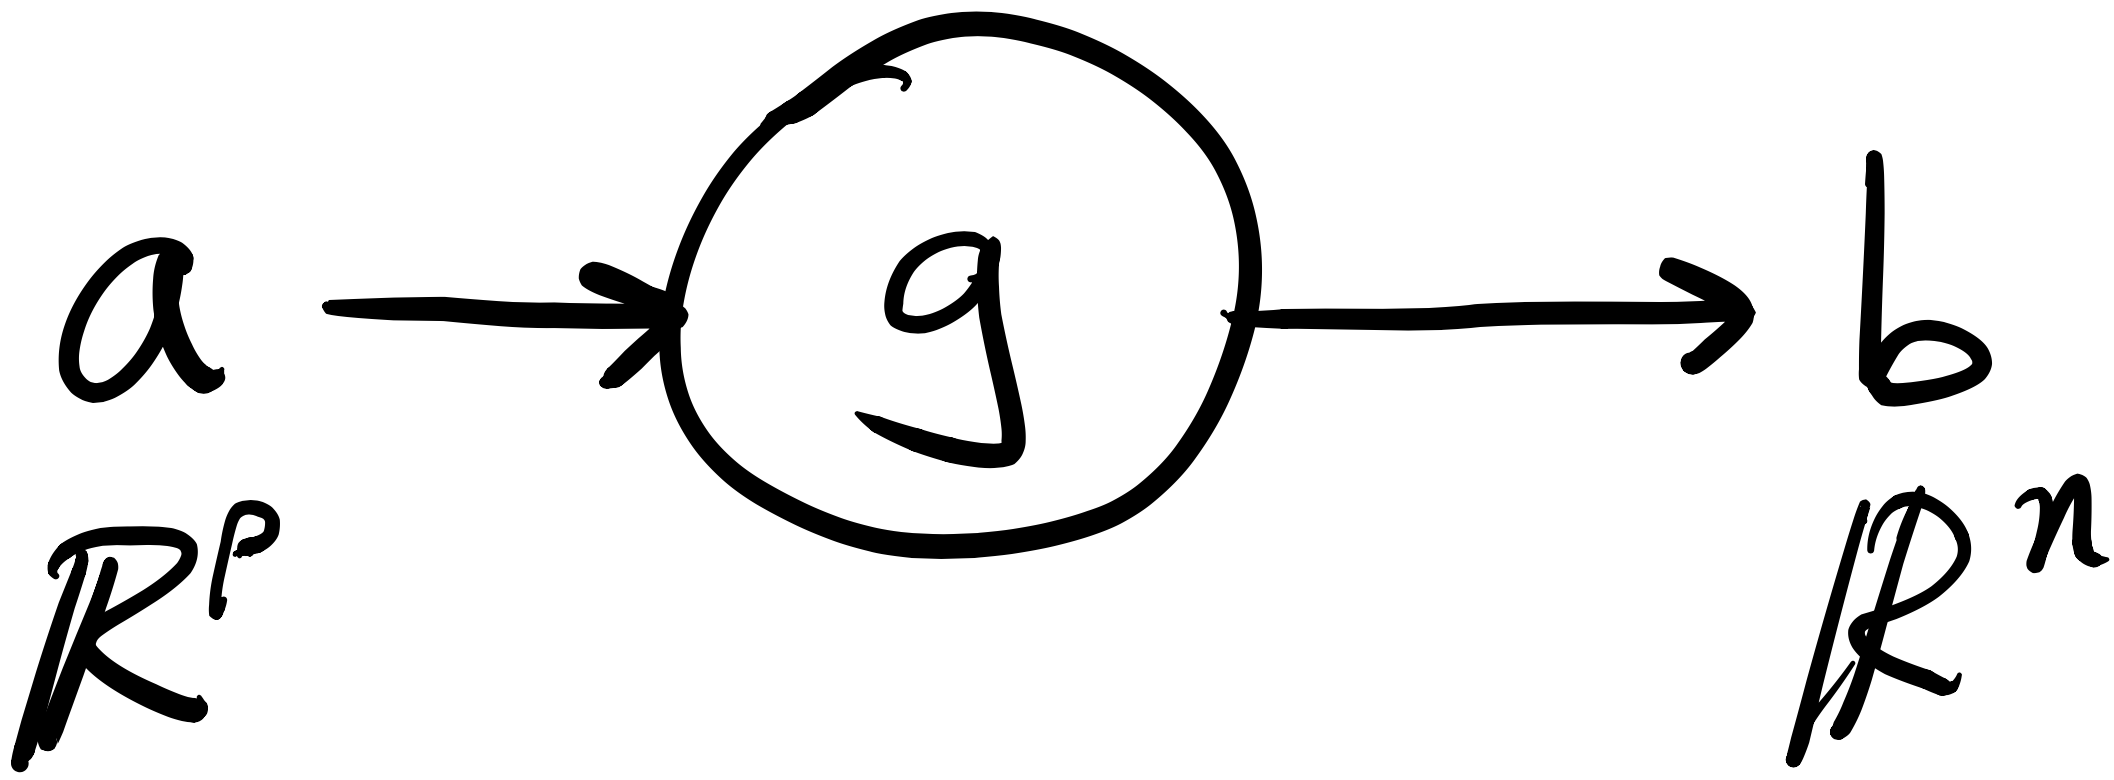
\includegraphics[scale=0.05]{figures/one-fn-comp-graph}

\column{.5\textwidth}
\begin{itemize}
\item Broken out into components:
\end{itemize}
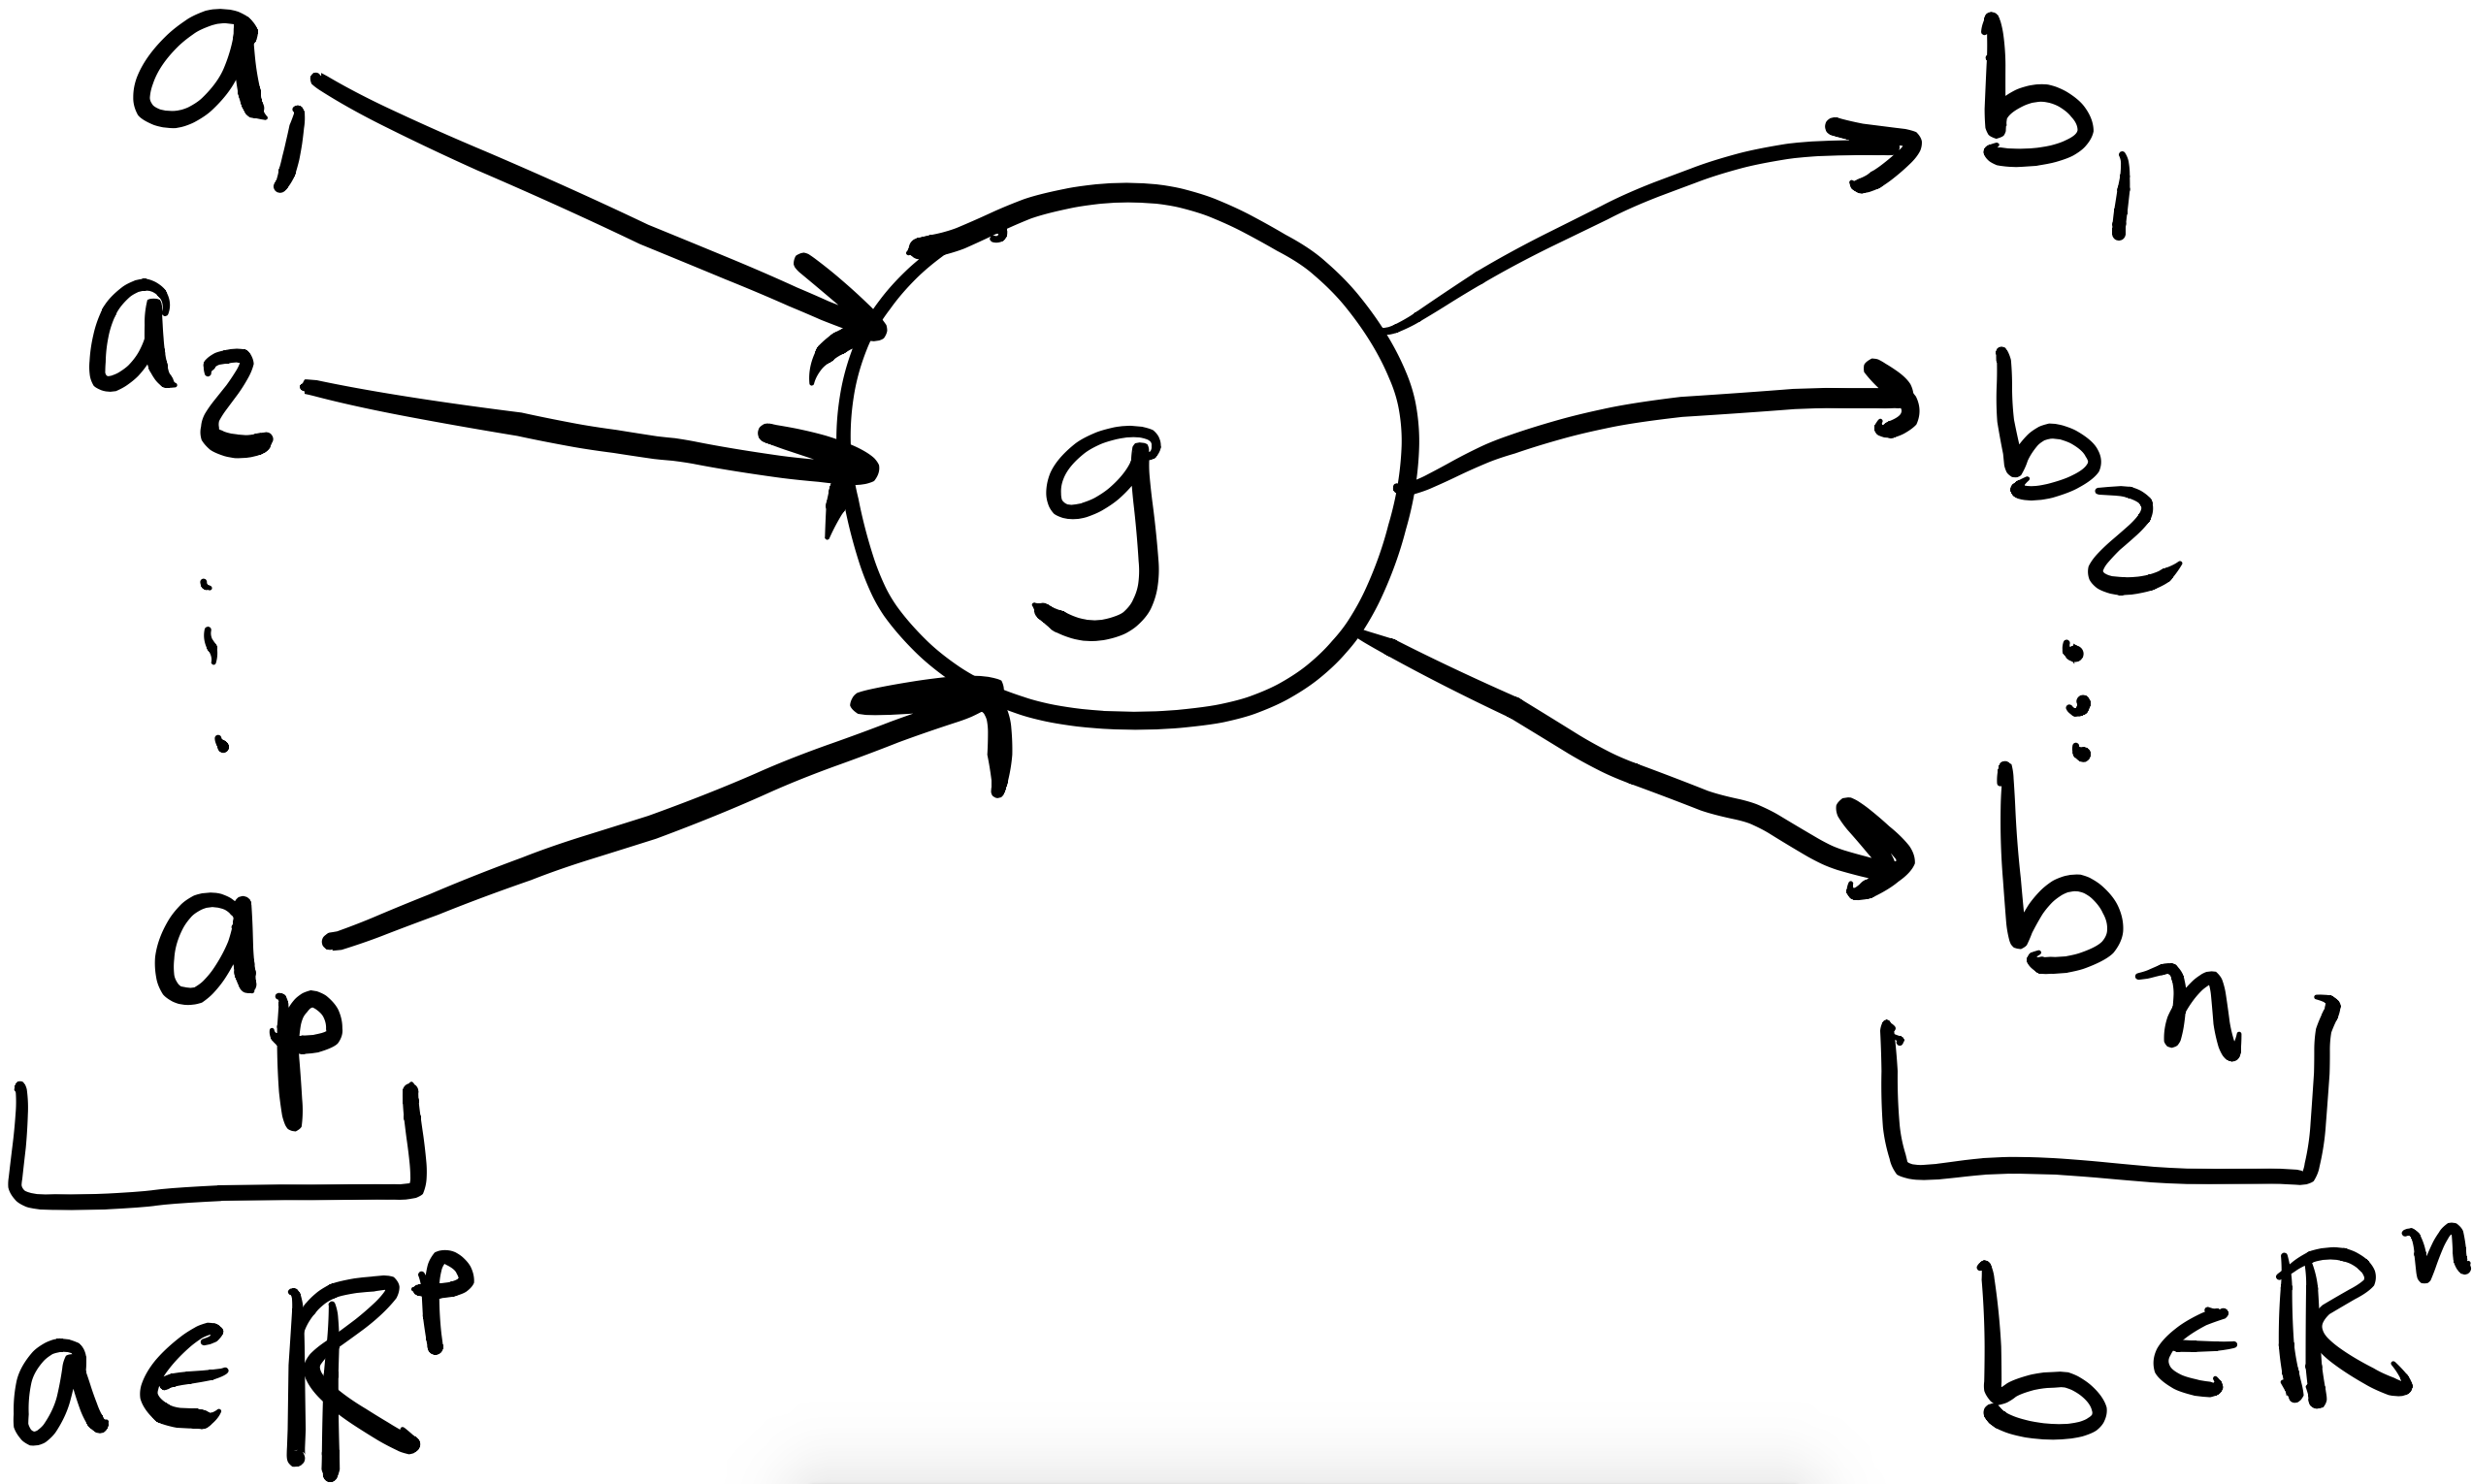
\includegraphics[scale=0.05]{figures/one-fn-comp-graph-partials}
\end{columns}

    \pdfnote{
CG is a useful abstraction for gradient computation on neural networks and implement neural network softwares.
    }
\end{frame}

\begin{frame}
{Compose multiple functions}
    {(adpated from David Rosenberg's slides)}

Compose two functions $g:\BR^{p}\to\BR^{n}$ and $f:\BR^{n}\to\BR^{m}$: $c=f(g(a))$
\\
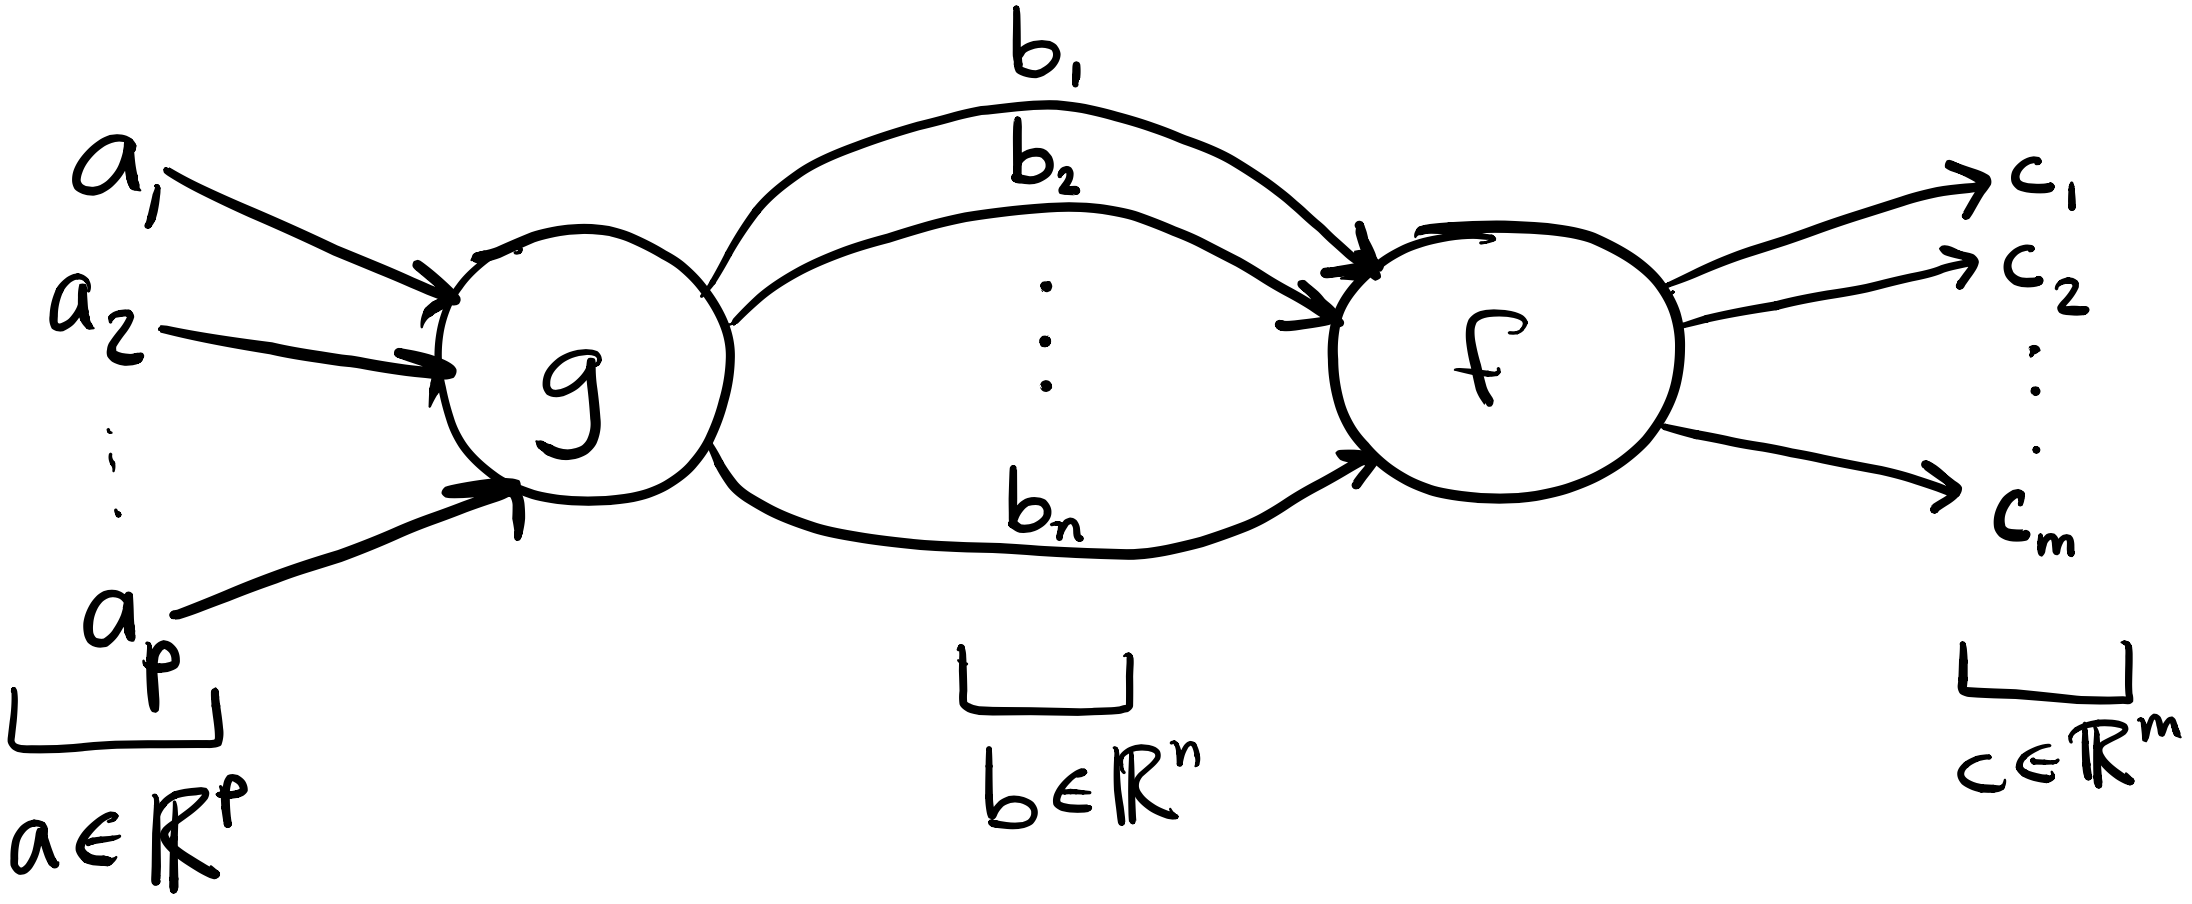
\includegraphics[height=2.5cm]{figures/two-fn-comp-graph-partials}
\\

\pause
\begin{itemize}
\item Derivative: How does change in $a_j$ affect $c_i$?
    \pause
$$
\frac{\partial c_{i}}{\partial a_{j}}={\color{blue}\sum_{k=1}^{n}}
{\color{red} \frac{\partial c_{i}}{\partial b_{k}}\frac{\partial b_{k}}{\partial a_{j}}} .
$$
        \vspace{-1em}
\pause
\item Visualize the multivariable \textbf{chain rule}:
\begin{itemize}
\item \textcolor{blue}{Sum} changes induced on all paths from $a_j$ to $c_i$.
\item Changes on one path is the {\color{red}product} of changes across each node.
\end{itemize} 
\end{itemize}
\end{frame}

\begin{frame}
    {Computation graph example}
    {(adpated from David Rosenberg's slides)}

    \begin{columns}
\column{.45\textwidth}
        \onslide<1->{
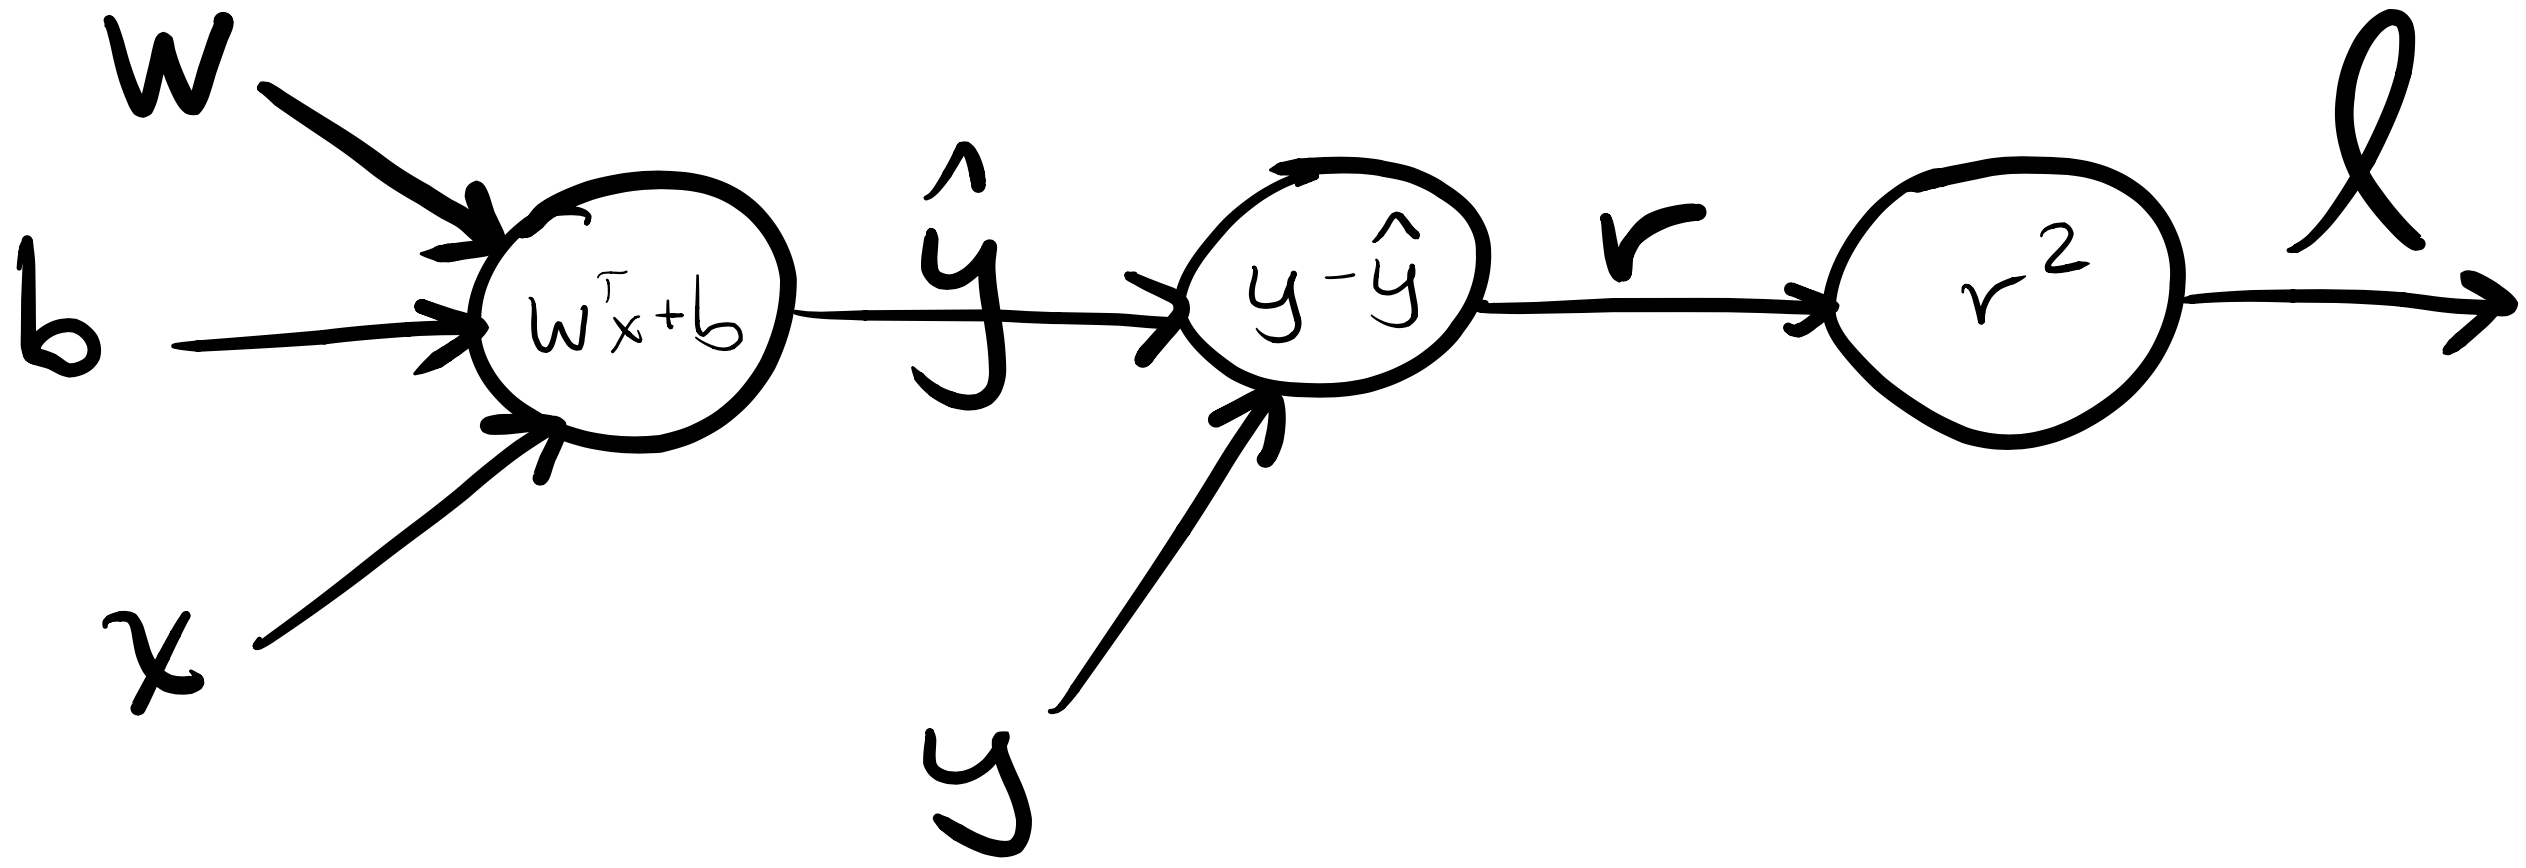
\includegraphics[width=1\textwidth]{figures/linear-sqr-loss-comp-graph}
        \\ (What is this graph computing?)
    }


\column{.45\textwidth}

\begin{eqnarray*}
    \onslide<4->{
        \green{\frac{\partial\ell}{\partial r}} & = & 2r\\
    \blue{\frac{\partial\ell}{\partial\hat{y}}} & = & \green{\frac{\partial\ell}{\partial r}}\frac{\partial r}{\partial\hat{y}}=\left(2r\right)(-1)=-2r\\
    }
    \onslide<2->{
        \frac{\partial\ell}{\partial b} & = & \blue<3->{\frac{\partial\ell}{\partial\hat{y}}}\frac{\partial\hat{y}}{\partial b}=\left(-2r\right)(1)=-2r\\
    \frac{\partial\ell}{\partial w_{j}} & = & \blue<3->{\frac{\partial\ell}{\partial\hat{y}}}\frac{\partial\hat{y}}{\partial w_{j}}=\left(-2r\right)x_{j}=-2rx_{j}
    }
\end{eqnarray*}
\end{columns}
    \pdfnote{Our goal is to compute del l over del w and b which are our params. We can directly compute them or follow this order.}
    \pdfnote{However, note that there is repeated computation}

    \medskip
    \onslide<3->{
    Computing the derivatives in certain order allows us to save compute!
    }

\end{frame}

\begin{frame}
    {Backpropogation}
    Backpropogation = chain rule + dynamic programming on a computation graph

    \pause
    Forward pass
\begin{itemize}
\item \textbf{Topological order}: every node appears before its children
\item For each node, compute the output given the input (from its parents).
\end{itemize}
\begin{center}
\begin{tikzpicture}[shorten >=1pt]
      	\tikzstyle{unit}=[draw,shape=circle,minimum size =1cm]

		\node (start) at (0,1){$\ldots$};
       	\node[unit](i) at (3,1){$f_i$};
        	\node[unit](j) at (6,1){$f_j$};
        	\node (end) at (9,1){$\ldots$};

        	\draw[->] (i) -- (j);
        	\draw[->] (start) -- (i);
        	\draw[->] (j) -- (end);
		
		\begin{scope}[transform canvas={yshift=-.7em}]
		\draw [->, Green, line width=0.05cm, shorten <=1mm, shorten >=1mm] (start) -- node {} (i);
  		\draw [->, Green, line width=0.05cm, shorten <=1mm, shorten >=1mm] (i) -- node {} (j);
  		\draw [->, Green, line width=0.05cm, shorten <=1mm, shorten >=1mm] (j) -- node {} (end);
		\end{scope}
		
		\begin{scope}[transform canvas={yshift=-1.4em}]
		\node (i-in) [right=0.2cm of start] {$a$};
		\node (j-in) [right=0.2cm of i] {$b=f_i(a)$};
		\node (j-out) [right=0.2cm of j] {$c=f_j(b)$};
		\end{scope}
\end{tikzpicture}
\end{center}
    \vspace{3em}
\end{frame}

\begin{frame}
    {Backpropogation}
    Backward pass
\begin{itemize}
\item \textbf{Reverse topological order}: every node appear after its children
\item For each node, compute the partial derivative of its output w.r.t. its input, multiplied by the partial derivative from its children (chain rule).
\end{itemize}
\begin{center}
\begin{tikzpicture}[shorten >=1pt]
      	\tikzstyle{unit}=[draw,shape=circle,minimum size =1cm]

		\node (start) at (0,1){$\ldots$};
       	\node[unit](i) at (3,1){$f_i$};
        	\node[unit](j) at (6,1){$f_j$};
        	\node (end) at (9,1){$\ldots$};

        	\draw[->] (i) -- (j);
        	\draw[->] (start) -- (i);
        	\draw[->] (j) -- (end);
		
		\begin{scope}[transform canvas={yshift=-.7em}]
		\draw [->, Green, line width=0.05cm, shorten <=1mm, shorten >=1mm] (start) -- node {} (i);
  		\draw [->, Green, line width=0.05cm, shorten <=1mm, shorten >=1mm] (i) -- node {} (j);
  		\draw [->, Green, line width=0.05cm, shorten <=1mm, shorten >=1mm] (j) -- node {} (end);
		\end{scope}
		
		\begin{scope}[transform canvas={yshift=-1.4em}]
		\node (i-in) [right=0.2cm of start] {$a$};
		\node (j-in) [right=0.2cm of i] {$b=f_i(a)$};
		\node (j-out) [right=0.2cm of j] {$c=f_j(b)$};
		\end{scope}
		
		\begin{scope}[transform canvas={yshift=-2.5em}]
		\draw [<-, red, line width=0.05cm, shorten <=1mm, shorten >=1mm] (start) -- node {} (i);
  		\draw [<-, red, line width=0.05cm, shorten <=1mm, shorten >=1mm] (i) -- node {} (j);
%  		\draw [<-, red, line width=0.05cm, shorten <=1mm, shorten >=1mm] (j) -- node {} (end);
		\end{scope}
		
		\begin{scope}[transform canvas={yshift=-3.4em}]
		\node (i-out) [left=0.2cm of i] {$g_i=g_j \cdot \frac{\partial b}{\partial a} = \frac{\partial J}{\partial a}$};
		\node (j-out) [left=0.2cm of j] {$g_j=\frac{\partial J}{\partial b}$};
		\end{scope}
\end{tikzpicture}
\end{center}
    \pdfnote{Each node takes the gradient passed from its child. If there are multiple children, then the gradients are added together. Then it computes the dot product of the gradient from its children and its local gradient. And pass the result to its parents.}
\end{frame}

\begin{frame}
    {Summary}
    Key idea in neural nets: feature/representation learning 

    Building blocks:\\
    \begin{itemize}
        \item Input layer: raw features (no learnable parameters)
        \item Hidden layer: perceptron + nonlinear activation function
        \item Output layer: linear (+ transformation, e.g. softmax)
    \end{itemize}

    Optimization:\\
    \begin{itemize}
        \item Optimize by SGD (implemented by back-propogation)
        \item Objective is non-convex, may not reach a global minimum
    \end{itemize}
\end{frame}

\section{Recurrent neural networks}

\begin{frame}
    {Overview}
    
    \textbf{Problem setup}: given an input sequence, come up with a (neural network) model that outputs a representation of the sequence for downstream tasks (e.g., classification)
    \pause

    \textbf{Key challenge}: how to model interaction among words?

    \pause
    \textbf{Approach}:\\
    \begin{itemize}
        \item Aggregation (pooling word embeddings)
        \item Recurrence
        \item Self-attention
    \end{itemize}
\end{frame}

\begin{frame}
    {Feed-forward neural network for text classification}
    %Encode a \emph{fixed-length} input using feed-forward NN (MLP):
    \begin{figure}
        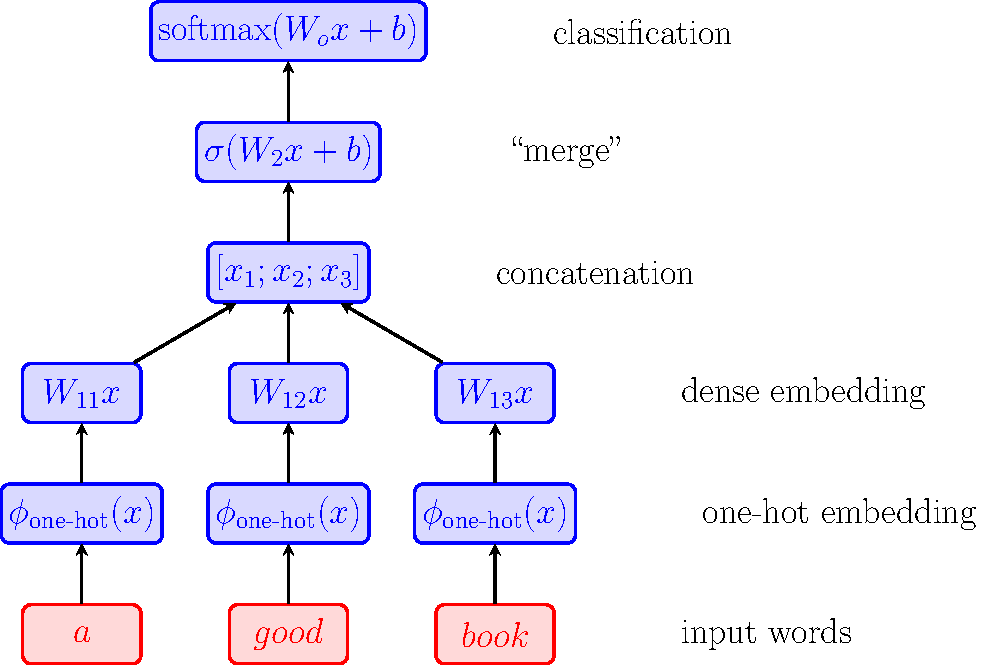
\includegraphics[height=5cm]{figures/fflm}
    \end{figure}
    \pause
    \think{
        Where is the interaction between words modeled?\\
        How to adapt the network to handle sequences with arbitrary length?}
    \pdfnote{
        Word embedding can encode any feature about a single words, e.g. prefix/suffix, POS tags etc.
        The merge step allows for interaction among words in the context, e.g. bigram.
    }
\end{frame}

\begin{frame}
    {Recurrent neural networks}
    \begin{itemize}
        \item \textbf{Goal}: compute representation of sequence $x_{1:T}$ of \blue{varying lengths}

        \item \textbf{Idea}: combine new symbols with previous symbols \blue{recurrently} %by modeling the \blue{temporal dynamics}
            \pdfnote{Read the sequence from left to right, update the representation with each new word read}
%    $$
% h_t = \sigma(\underbrace{W_{hh}h_{t-1}}_{\textstyle\text{previous state}}+
% \underbrace{W_{ih}x_t}_{\textstyle\text{new input}} + b_h)
% \;.
%    $$
    \pdfnote{
        RNN is a model for sequence data.
        We add a piece of new information at each time step.
    Specifically, we maintain a representation of the current state, which summarizes the context until the current time step.
    To compute the current state, we take the previous state and combine it with the new input.
    }

    \pause
    \begin{itemize}
        %\item Set the initial state $h_0$ to some deterministic (or learned) value
        \item Update the representation, i.e. \textbf{hidden states} $h_t$, recurrently
    $$
    h_t = f(h_{t-1}, x_t)
    $$
    \vspace{-1em}
            \begin{itemize}
            \item Output from previous time step is the input to the current time step
            \item Apply the same transformation $f$ at each time step
            \end{itemize}
    \vspace{1em}
    \begin{figure}
        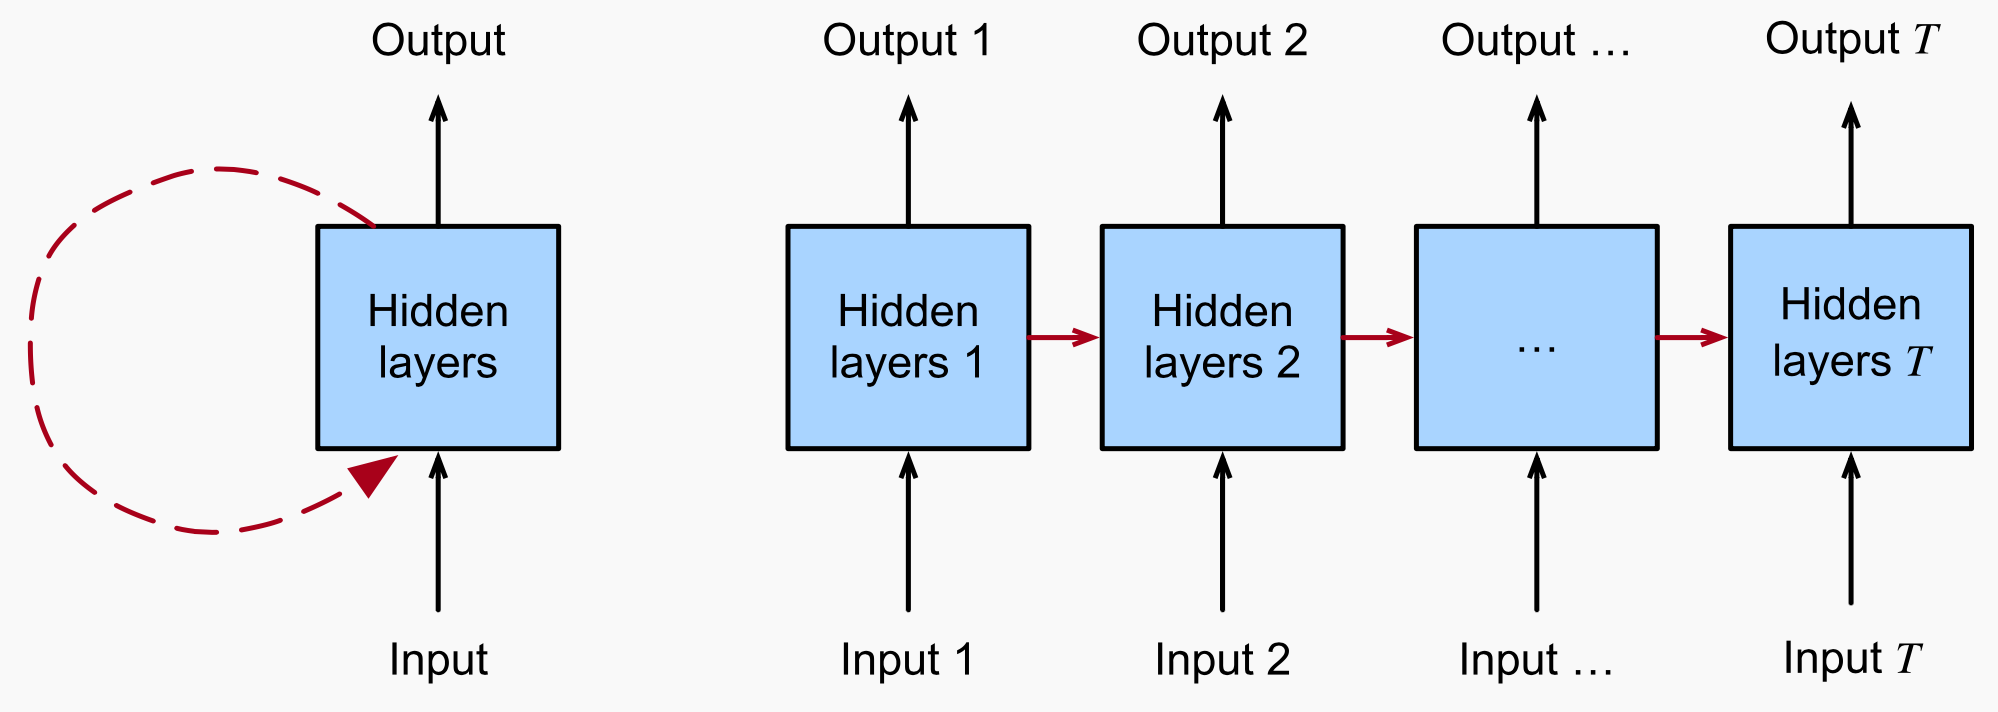
\includegraphics[height=2.5cm]{figures/rnn-concept}
        \caption{9.1 from \href{https://d2l.ai/chapter_recurrent-neural-networks}{d2l.ai}}
    \end{figure}
    \end{itemize}
    \end{itemize}

\end{frame}

\begin{frame}
    {Forward pass}
    \begin{columns}
        \begin{column}{0.6\columnwidth}
    \begin{figure}
        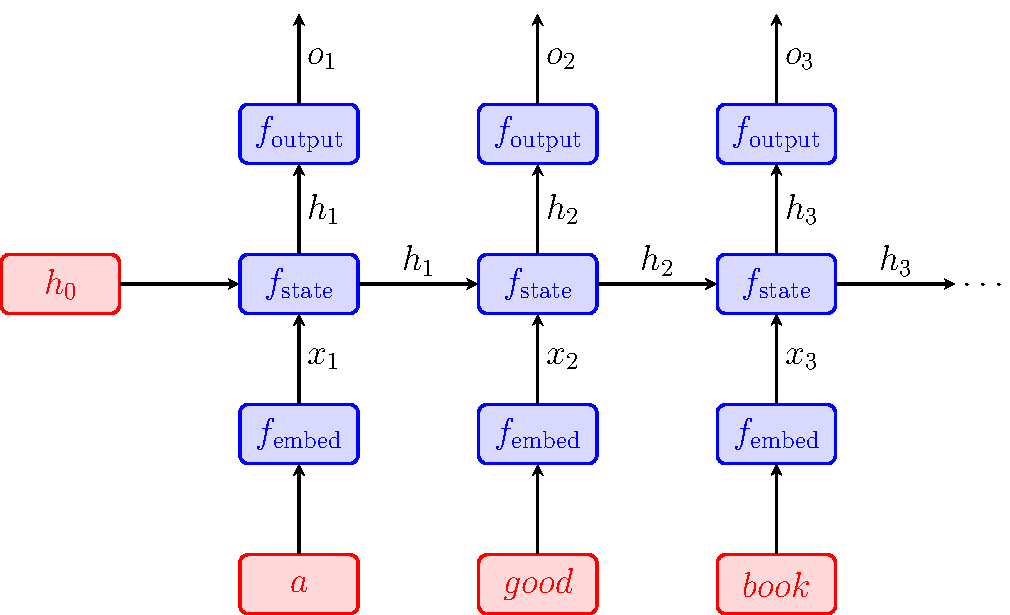
\includegraphics[height=5cm]{figures/rnn}
    \end{figure}
        A deep neural network with shared weights in each layer
        \end{column}
        \onslide<2->{
        \begin{column}{0.4\columnwidth}
            \begin{align*}
                x_t &= f_{\text{embed}}(s_t) \\
                &= W_e\phi_{\text{one-hot}}(s_t)\\[1em]
                \onslide<3->{
                h_{t} &= f_{\text{state}}(x_t, h_{t-1}) \\
                &= \sigma(W_{hh}h_{t-1} + W_{ih}x_t + b_h) \\[1em]
                }
                \onslide<4->{
                    o_t &= f_{\text{output}}(h_t) \\
                &= \mathrm{softmax}(W_{ho}h_t + b_o) \\
                & \text{(a distribution over classes)}
                }
            \end{align*}


            \onslide<5->{\think{Which computation can be parallelized?}}
        \end{column}
        }
    \end{columns}
    \pdfnote{
        The recurrent unit has two learnable matrices to combine prev state and input.
    }
    \pdfnote{
        The output o is a real vector, and we can take that as a feature vector of each word with the left context,
        which can be then used to predict the next word.
    }
\end{frame}

\begin{frame}
    {Loss functions on RNNs}
    
    {\bf Sequence labeling and language modeling}:\\
    \begin{itemize}
        \item Input: $x_1, \ldots, x_T$ (a sequence of tokens)
        \item Output: $y_1, \ldots, y_T$ (e.g., POS tags, next words)
        \item Loss function: $\sum_{i=1}^T \ell(y_t, o_t)$
            \begin{itemize}
                \item NLL loss: $\sum_{i=1}^T -\log o_t[y_t]$
            \end{itemize}
    \end{itemize}

    \pause
    {\bf Text classification}:\\
    \begin{itemize}
        \item Input: $x_1, \ldots, x_T$
        \item Output: $y\in \pc{1,\ldots, K}$ ($K$ classes)
        \item Loss function: $\ell(y, f_{\text{output}}(\blue{\mathrm{pool}}(h_1, \ldots, h_T)))$
            \begin{itemize}
                \item Can use last hidden state or mean of all hidden states
            \end{itemize}
    \end{itemize}

\end{frame}

\begin{frame}
    {Backward pass}
    Given the loss $\ell(y_t, o_t)$, compute the gradient with respect to $W_{hh}$.
    $$
    \frac{\pt\ell_t}{\pt W_{hh}} = \pause \frac{\pt\ell_t}{\pt o_t} \frac{\pt o_t}{\pt h_t} \frac{\pt h_t}{\pt W_{hh}}
    $$

    \pause
    Computation graph of $h_t$: $h_t = \sigma(W_{hh}h_{t-1} + W_{hi}x_t + b)$
    \vspace{10em}
\end{frame}

\begin{frame}
    {Backpropagation through time}
    
    Problem with standard backpropagation:\\
    \begin{itemize}
        \item Gradient involves \red{repeated multiplication of $W_{hh}$}
        \item Gradient will \red{vanish / explode} (depending on the eigenvalues of $W_{hh}$)
    \end{itemize}

    \pause
    Quick fixes:\\
    \begin{itemize}
        \item Reduce the number of repeated multiplication: truncate after $k$ steps ($h_{t-k}$ has no influence on $h_t$)
        \item Limit the norm (or value) of the gradient in each step: gradient clipping (can only mitigate explosion)
    \end{itemize}
\end{frame}

\begin{frame}
    {Long-short term memory (LSTM)}

    \textbf{Vanilla RNN}: always update the hidden state\\
    \begin{itemize}
        \item Cannot handle long range dependency due to gradient vanishing 
    \end{itemize}
    \pause

    \textbf{LSTM}: learn when to update the hidden state\\
    \begin{itemize}
        \item First successful solution to the gradient vanishing and explosion problem 
    \end{itemize}
    \pause

    Key idea is to use a \textbf{gating mechanism}: multiplicative weights that modulate another variable \\
    \begin{itemize}
        \item How much should the new input affect the state?
        \item When to ignore new inputs?
        \item How much should the state affect the output? 
    \end{itemize}
\end{frame}

\begin{frame}
    {Long-short term memory (LSTM) parametrization}
    \begin{figure}
        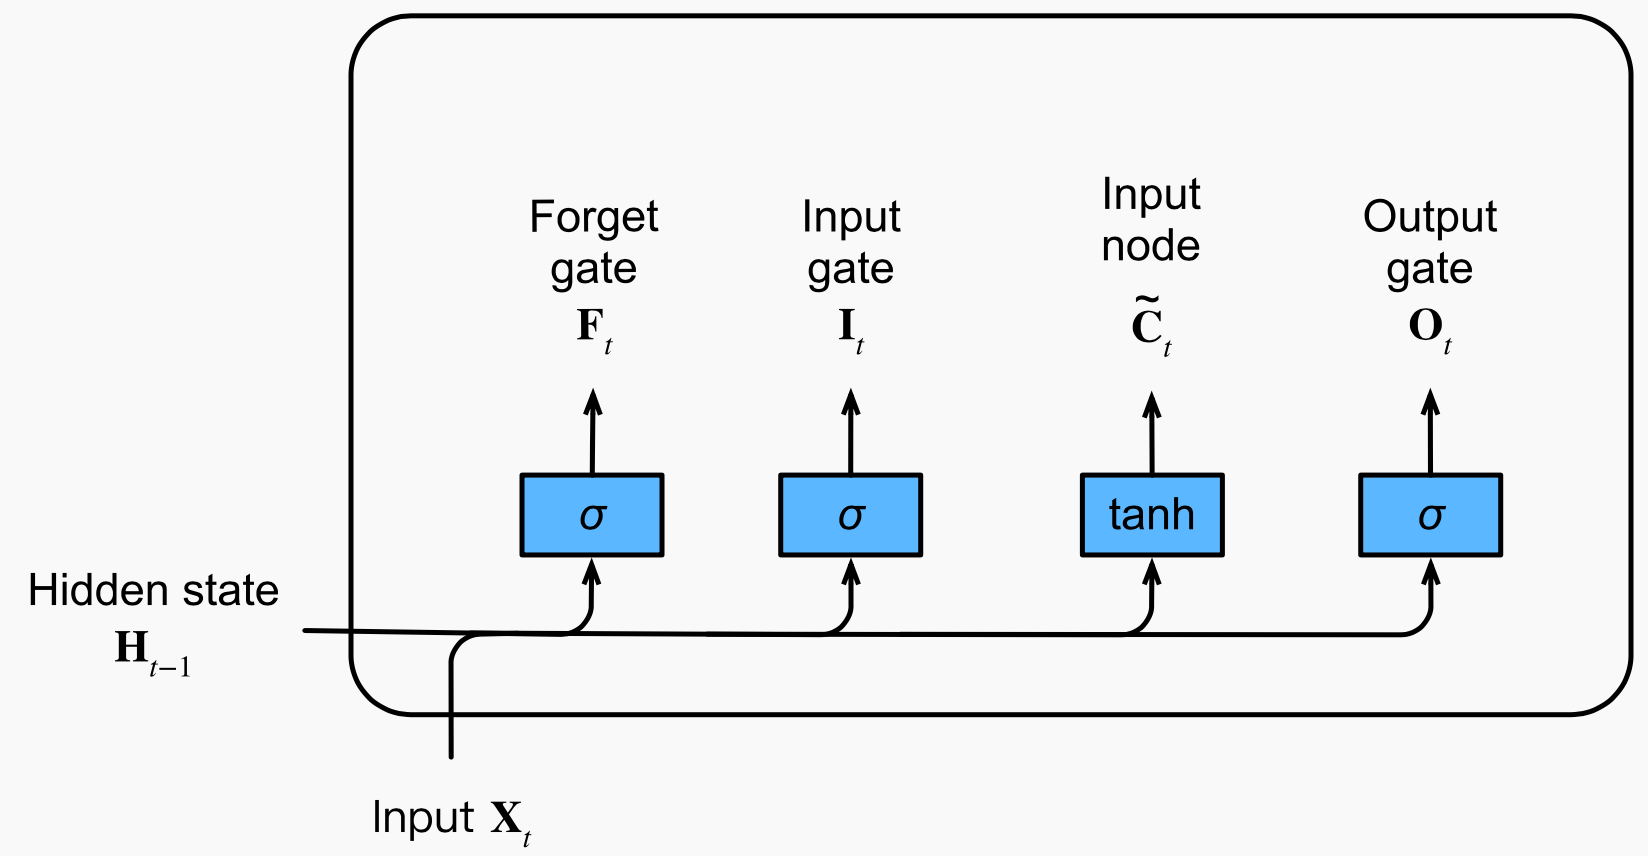
\includegraphics[height=4cm]{figures/lstm-1}
        \caption{10.1.2 from \href{https://d2l.ai/chapter_recurrent-modern/lstm.html}{d2l.ai}}
    \end{figure}
    \vspace{-1em}

    Update with the new input $x_t$ (same as in vanilla RNN)
    $$
    \tilde{c}_t = \tanh(W_{xc}x_t + W_{hc}h_{t-1} + b_c) \quad \text{\blue{new cell content}}
    $$

    \pause\vspace{-1ex}
    Should we update with the new input $x_t$?
\end{frame}

\begin{frame}
    {Long-short term memory (LSTM) parametrization}
    \begin{figure}
        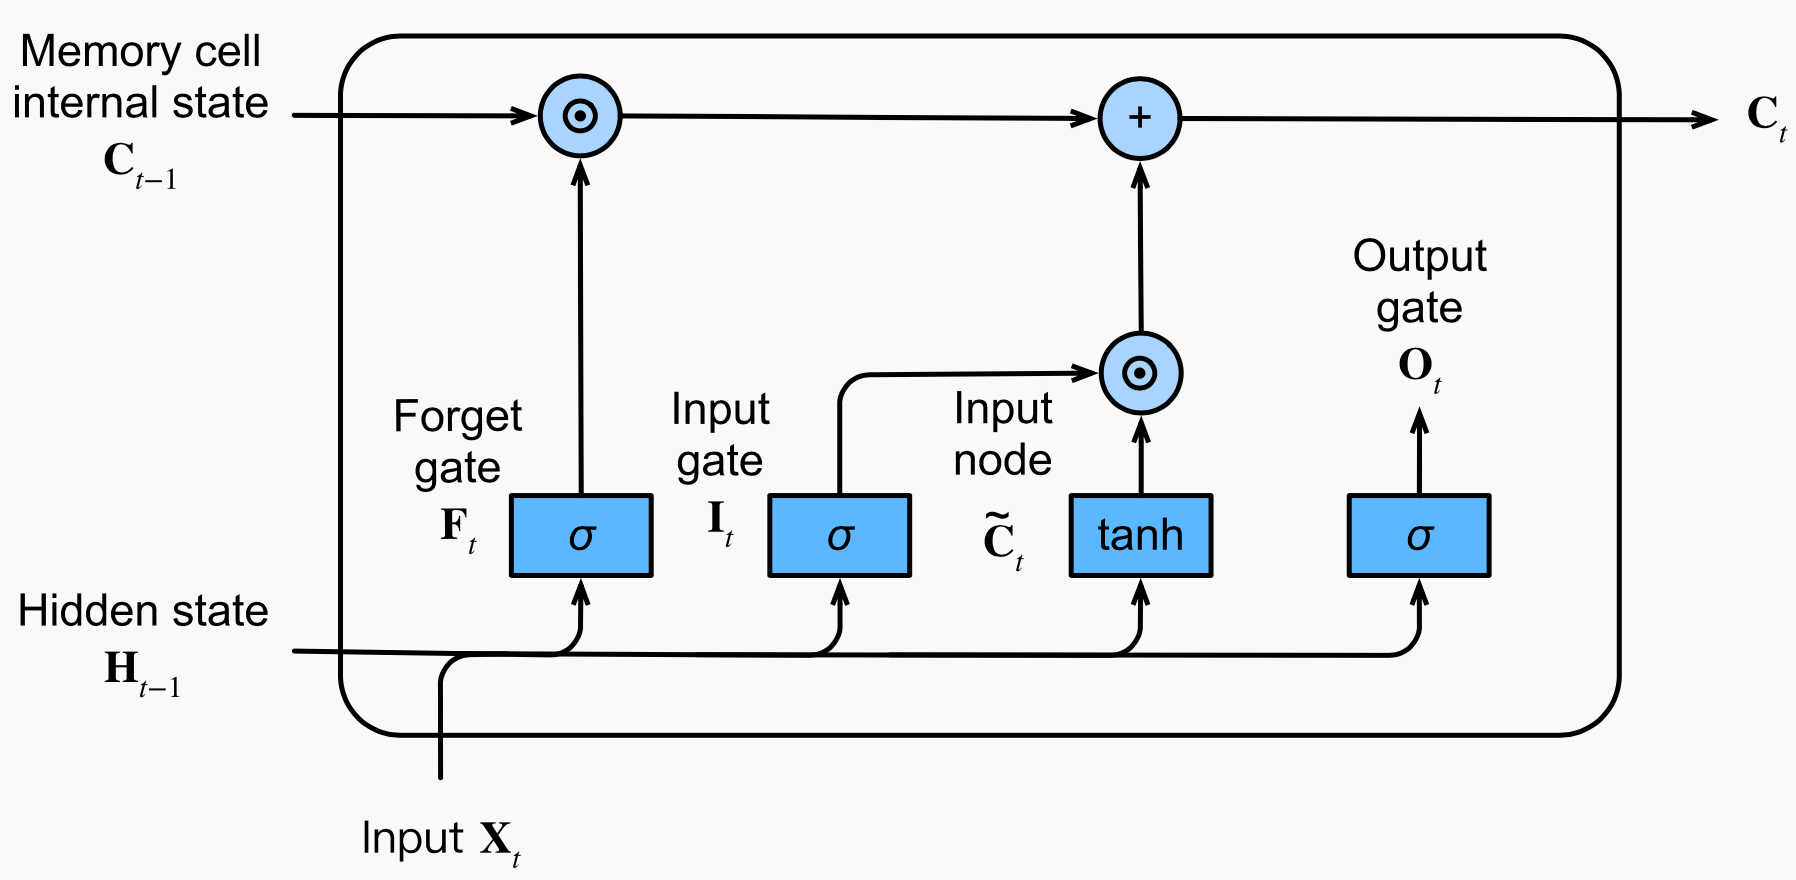
\includegraphics[height=4cm]{figures/lstm-2}
        \caption{10.1.3 from \href{https://d2l.ai/chapter_recurrent-modern/lstm.html}{d2l.ai}}
    \end{figure}
    \vspace{-1em}

    Choose between $\tilde{c}_t$ (\blue{update}) and $c_{t-1}$ (\red{no update}): 
    ($\odot$: elementwise product)
    $$
    \textbf{memory cell} \quad
    c_t = i_t \odot \tilde{c}_t + f_t \odot c_{t-1}
    $$

    \vspace{-1ex}
    \begin{itemize}
        \item $f_t$: proportion of the old state (\red{preserve $\uparrow$ or erase $\downarrow$ the old memory})
        \item $i_t$: proportion of the new state (\blue{write $\uparrow$ or ignore $\downarrow$ the new input})
        \item What is $c_t$ if $f_t=1$ and $i_t=0$?
            \pdfnote{$h_0$}
    \end{itemize}
\end{frame}

\begin{frame}
    {Long-short term memory (LSTM) parametrization}
    \begin{figure}
        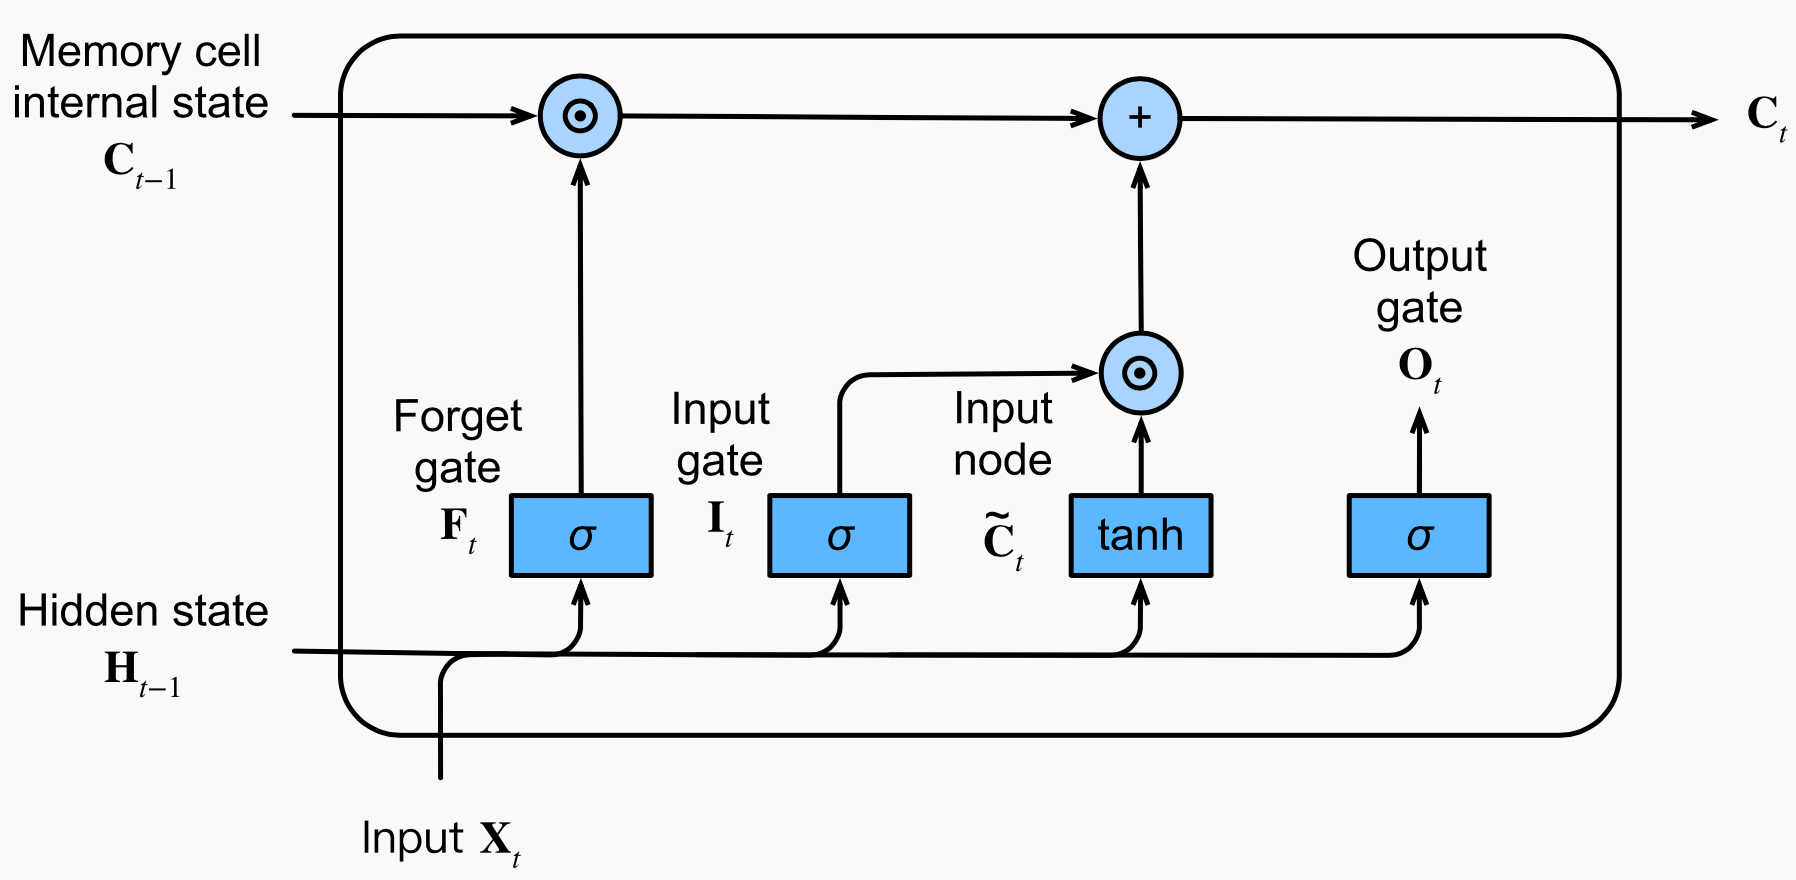
\includegraphics[height=4cm]{figures/lstm-2}
    \end{figure}

    Input gate and forget gate \blue{depends on data}:
            \begin{align*}
                i_t &= \text{sigmoid}(W_{xi}\blue{x_t} + W_{hi}h_{t-1} + b_i) \;,\\
                f_t &= \text{sigmoid}(W_{xf}\blue{x_t} + W_{hf}h_{t-1} + b_f) \;.
            \end{align*}
    Each coordinate is between 0 and 1.
\end{frame}

\begin{frame}
    {Long-short term memory (LSTM) parametrization}
    \begin{figure}
        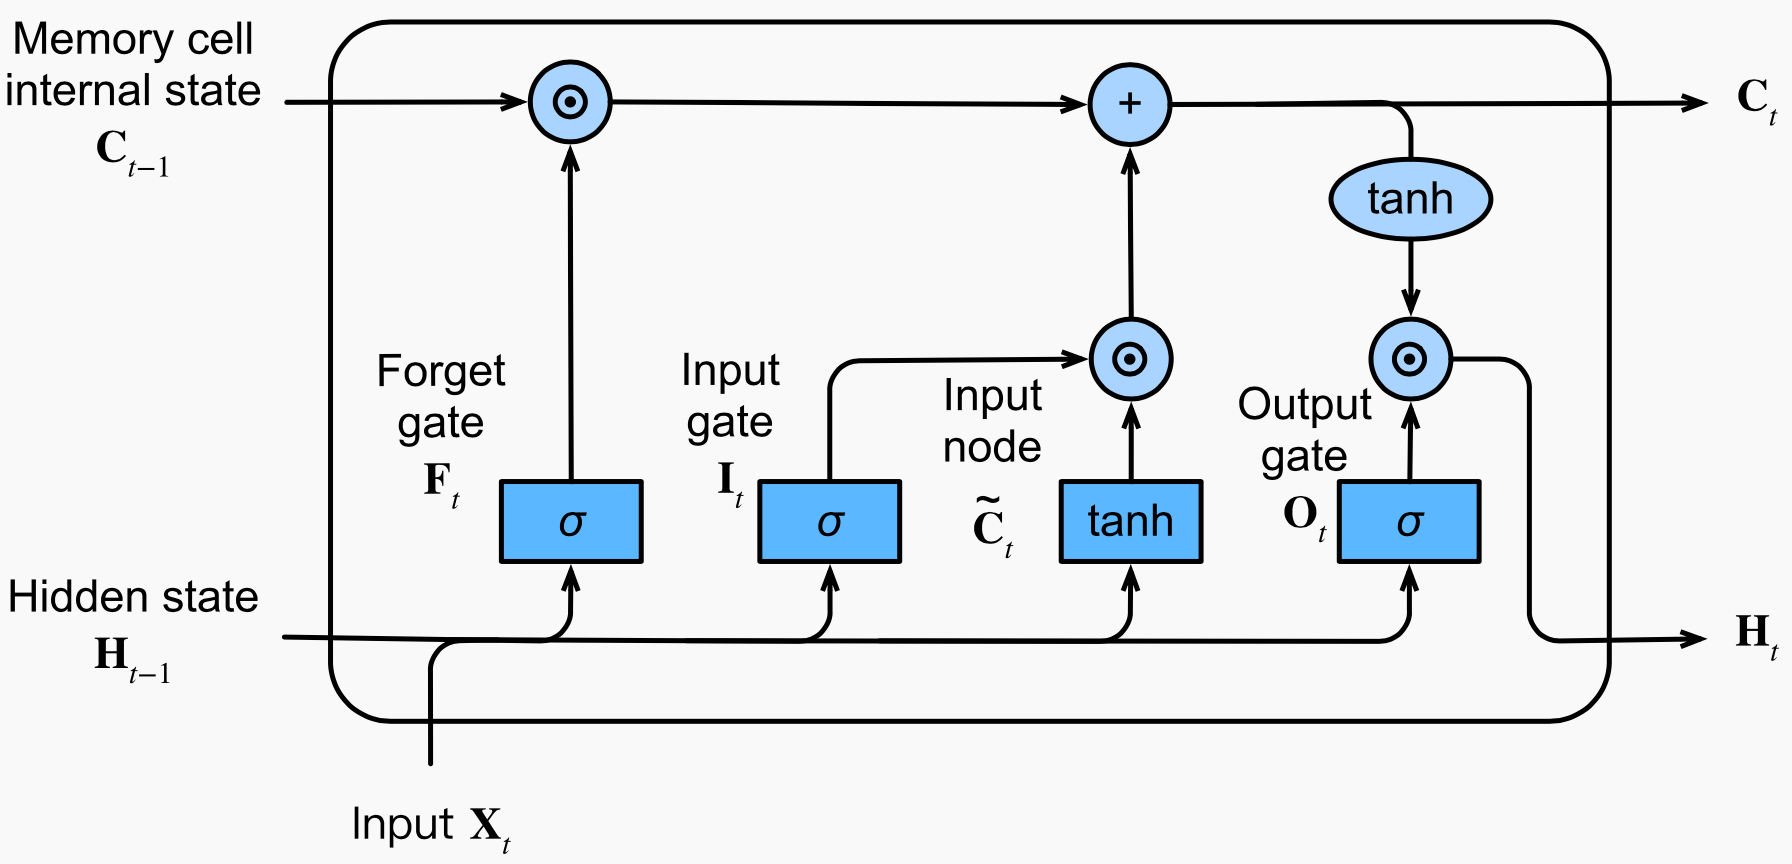
\includegraphics[height=4cm]{figures/lstm-3}
        \caption{10.1.4 from \href{https://d2l.ai/chapter_recurrent-modern/lstm.html}{d2l.ai}}
    \end{figure}
    How much should the memory cell state influence the rest of the network:
            \begin{align*}
 h_t &= o_t \odot c_t \\
 o_t &= \text{sigmoid}(W_{xo}x_t + W_{ho}h_{t-1} + b_o) 
            \end{align*}
    $c_t$ may accumulate information without impact the network if $o_t$ is close to 0
\end{frame}

\begin{frame}
    {How does LSTM solve gradient vanishing / explosion?}
    Intuition: gating allows the network to learn to control how much gradient should vanish.
    \begin{itemize}
        \item Vanilla RNN: gradient depends on repeated multiplication of the \blue{same weight matrix}
        \item LSTM: gradient depends on repeated multiplication of some quantity that depends on the data (values of \blue{input and forget gates})
        \item So the network can learn to reset or update the gradient depending on whether there is long-range dependencies in the data.
    \end{itemize}
    \pdfnote{
        How does it fix the gradient vanishing/exploding problem?
        With RNN our problem is that we end with repeated multiplication of the same matrix.
        Try compute del c(t) over del c(t-1).
        It still involves repeated multiplication of certain quantity, but it will depend on learned values that are different at each time step, specifically the input and forget gates.
        So the network can decide when to reset the gradient or to increase the gradient signal depending on whether there is long-range dependencies in the data.
    }
\end{frame}

\section{Self-attention}

\begin{frame}
    {Improve the efficiency of RNN}
    \begin{columns}
        \begin{column}{0.4\textwidth}
            \begin{figure}
                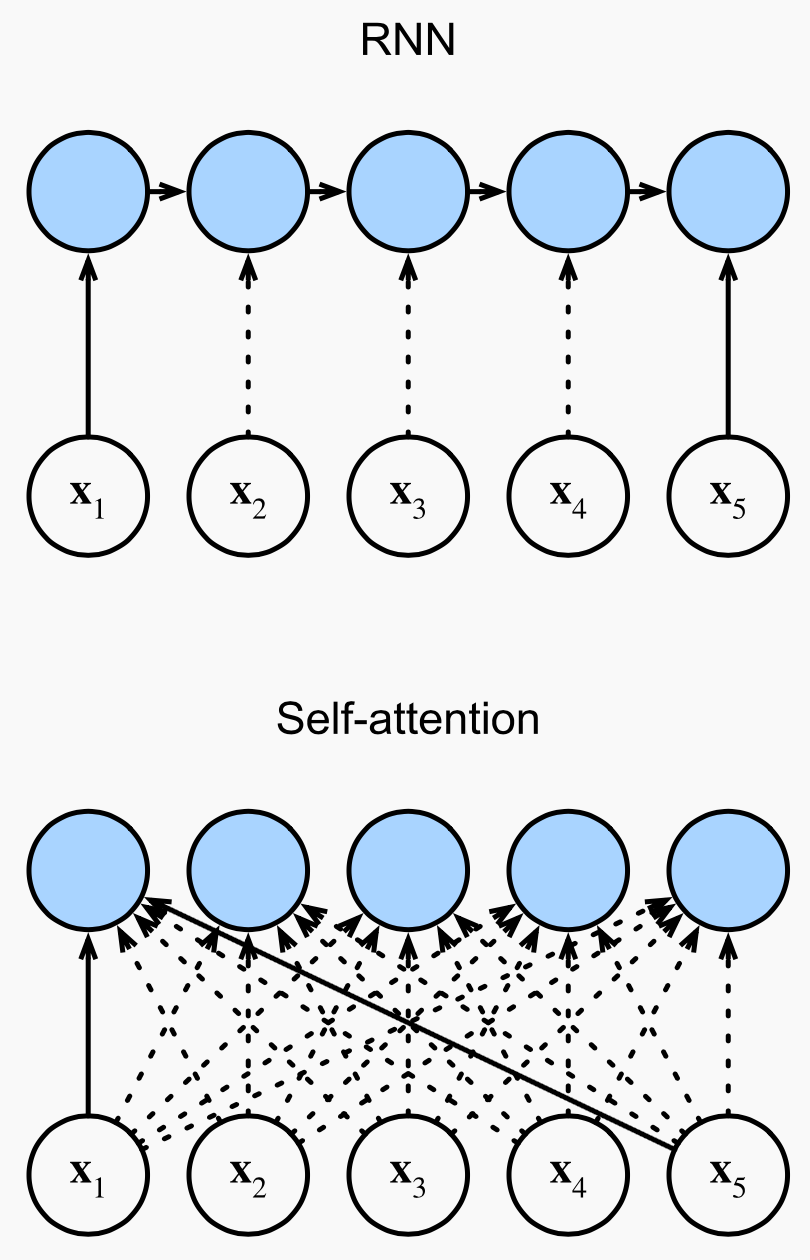
\includegraphics[width=4cm]{figures/rnn-attention-compare}
                \caption{11.6.1 from \href{https://d2l.ai/chapter_attention-mechanisms-and-transformers/self-attention-and-positional-encoding.html}{d2l.ai}}
            \end{figure}
        \end{column}
        \begin{column}{0.6\textwidth}
            Recall that our goal is to come up with a good respresentation of a sequence of words.\\
            \medskip

            RNN:\\
            \begin{itemize}
                \item Past words influence the sentence representation through \blue{recurrent update}
                \item \red{Sequential computation} $O(\text{sequence length})$, hard to scale
            \end{itemize}
            \medskip
            \pause

            Can we handle dependency more \green{efficiently}?\\
            \begin{itemize}
                \item \blue{Direct interaction} between any pair of words in the sequence
                \item Parallelizable computation 
            \end{itemize}
        \end{column}
    \end{columns}
\end{frame}

%\begin{frame}
%    {Model interaction between words}
%
%    {\em Time flies like an arrow}: Which word(s) is most related to ``time''?
%    \bigskip\pause
%
%    \begin{columns}
%        \begin{column}{0.4\textwidth}
%            A database approach: 
%            \begin{table}
%            \begin{tabular}{lll}
%                \textbf{query} & \textbf{keys} & \textbf{values} \\
%                &\texttt{arrow} & time \\
%                &\texttt{flies }& flies \\
%                &\texttt{like }& like \\
%                &\texttt{an }& an \\
%                time &\texttt{time}& arrow\\
%            \end{tabular}
%            \end{table}
%            \pause
%            Output: arrow
%        \end{column}
%        \pause
%        \begin{column}{0.6\textwidth}
%            Limitations:\\
%            \begin{wideitemize}
%                \item Relatedness should not be hard-coded
%                \item A word is related to multiple words in a sentence
%            \end{wideitemize}
%        \end{column}
%    \end{columns}
%\end{frame}

\begin{frame}
    {Model interaction between two variables}

    Given a {\bf query} and some context, how do we find relevant information from the context?

    Context representation:\\
    \begin{itemize}
        \item {\bf values}: content in the context 
        \item {\bf keys}: matching agaisnt the query to compute relevance
    \end{itemize}

    \pause
    Example:\\
    \begin{itemize}
        \item Reading comprehension: query=question, context=document
        \item Machine translation: query=text in French, context=text in English
    \end{itemize}
\end{frame}

\begin{frame}
    {Model interaction between words}
    \begin{figure}
        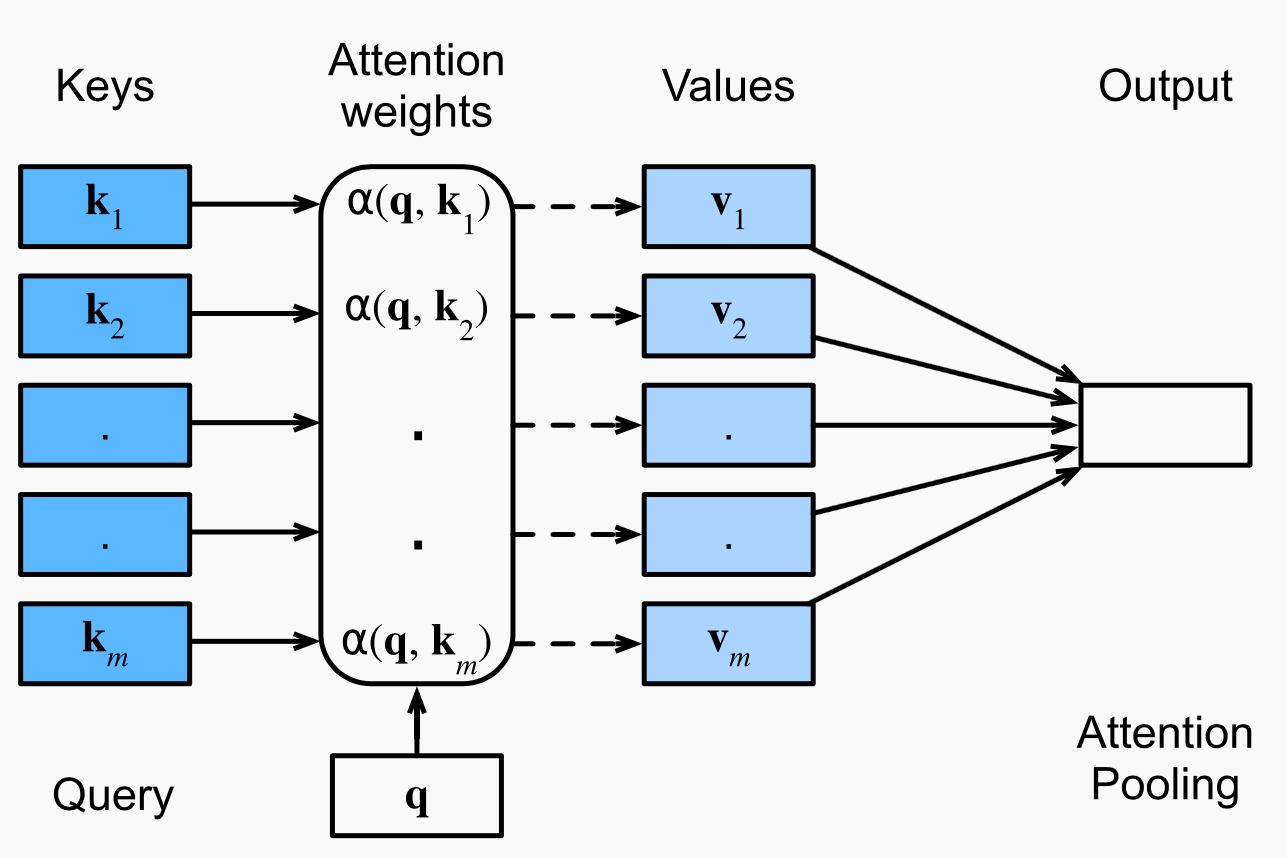
\includegraphics[height=5cm]{figures/qkv}
        \caption{11.1.1 from \href{https://d2l.ai/chapter_attention-mechanisms-and-transformers/queries-keys-values.html}{d2l.ai}}
    \end{figure}
    \vspace{-1em}
    \begin{itemize}
        \item \textbf{Attention weights} $\alpha(q, k_i)$: how strong is $q$ matched to $k_i$
        \item \textbf{Attention pooling}: combine $v_i$'s according to their ``relatedness'' to the query
    \end{itemize}
\end{frame}

\begin{frame}
    {Model interaction between words using a "soft" database}
    \begin{figure}
        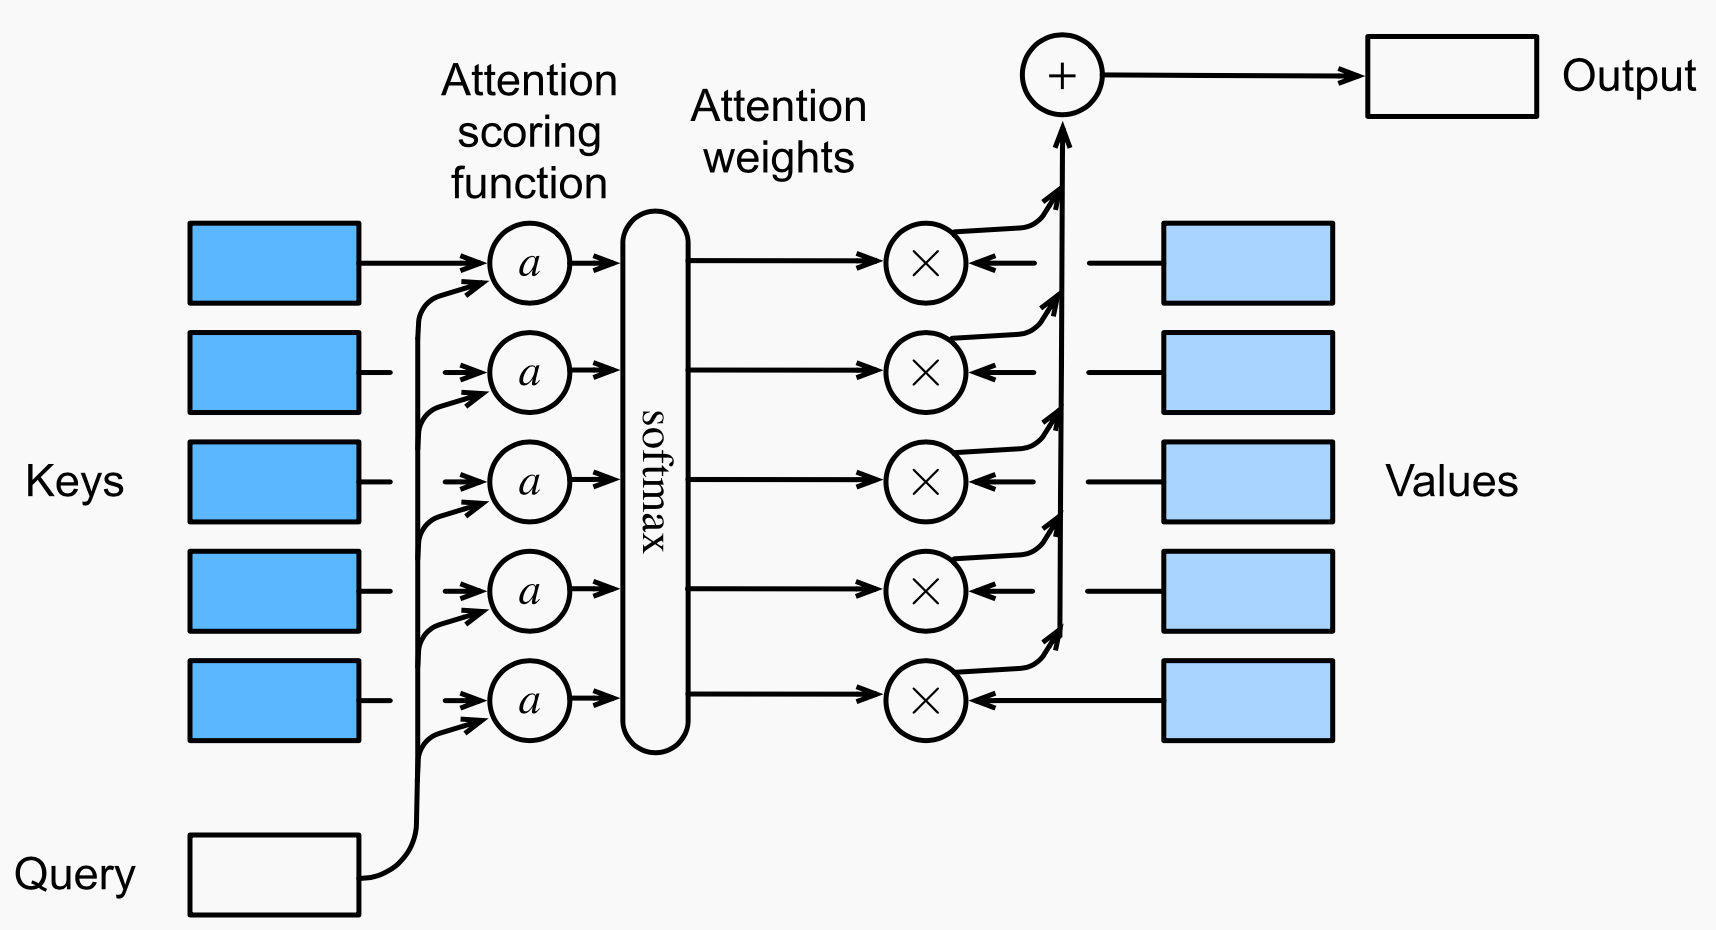
\includegraphics[height=5cm]{figures/qkv-2}
        \caption{11.3.1 from \href{https://d2l.ai/chapter_attention-mechanisms-and-transformers/attention-scoring-functions.html}{d2l.ai}}
    \end{figure}
    \vspace{-1em}
    \begin{itemize}
        \item Model {attention weights} as a distribution: $\alpha=\mathrm{softmax}(a(q,k_1),\ldots,a(q,k_m))$
        \item Output a weighted combination of values: $o_i = \sum_{i=1}^m \alpha(q,k_i) v_i$
    \end{itemize}
\end{frame}

\begin{frame}
    {Self-attention}

    Given two sets of objects (queries and context), attention allows us to model interactions between them.

    We can use it to model the interaction between each pair of words in a sentence.
    \pause

    \begin{figure}
        \begin{subfigure}{.5\textwidth}
        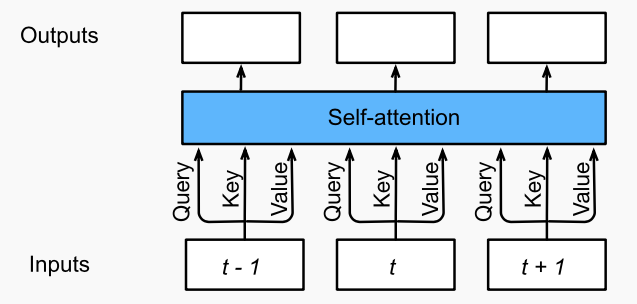
\includegraphics[height=3cm]{figures/self-attn}
        \end{subfigure}
        \begin{subfigure}{.4\textwidth}
        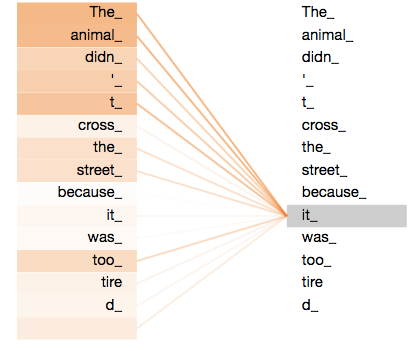
\includegraphics[height=3cm]{figures/self-attn-ex}
        \end{subfigure}
    \end{figure}
    \begin{itemize}[<+->]
        \item \blue{Input}: map each symbol to a query, a key, and a value (embeddings)
        \item \blue{Attend}: each word (as a query) interacts with all words (keys)
        \item \blue{Output}: \emph{contextualized} representation of each word (weighted sum of values)
    \end{itemize}
\end{frame}

\begin{frame}
    {Attention scoring functions}

    Design the function that measures relatedness between queries and keys:
    ${\alpha}= \mathrm{softmax}({\color{blue}{a}}({q}, k_1), \ldots, {\color{blue}{a}}({q}, k_m)) \quad\quad a\colon \BR^d \times \BR^d \to \BR$
    \pause

    \textbf{Dot-product attention}
    $$
    a(q, k) = q\cdot k
    $$
    \pause

    \textbf{Scaled dot-product attention}
    $$
    a(q, k) = q \cdot k / \sqrt{d} 
    $$
    \vspace{-3em}
    \begin{itemize}
        \item $\sqrt{d}$: dimension of the key vector
        \item Avoids large attention weights that push the softmax function into regions of small gradients
    \end{itemize}
    \pause

    \textbf{MLP attention}
    $$
    a(q, k) = u^T \tanh(W[q;k]) 
    $$
\end{frame}

\begin{frame}
    {Multi-head attention: motivation}
    \begin{center}
        \textit{Time flies like an arrow}
    \end{center}
    \begin{wideitemize}
        \item Each word attends to all other words in the sentence
        \item Which words should ``like'' attend to?
            \pause
            \begin{itemize}
                \item Syntax: ``flies'', ``arrow'' (a preposition)
                \item Semantics: ``time'', ``arrow'' (a metaphor)
            \end{itemize}
        \pause
        \item We want to represent different roles of a word in the sentence: need more than a single embedding
        \item Instantiation: multiple self-attention modules
    \end{wideitemize}
\end{frame}

\begin{frame}
    {Multi-head attention}
    \begin{figure}
        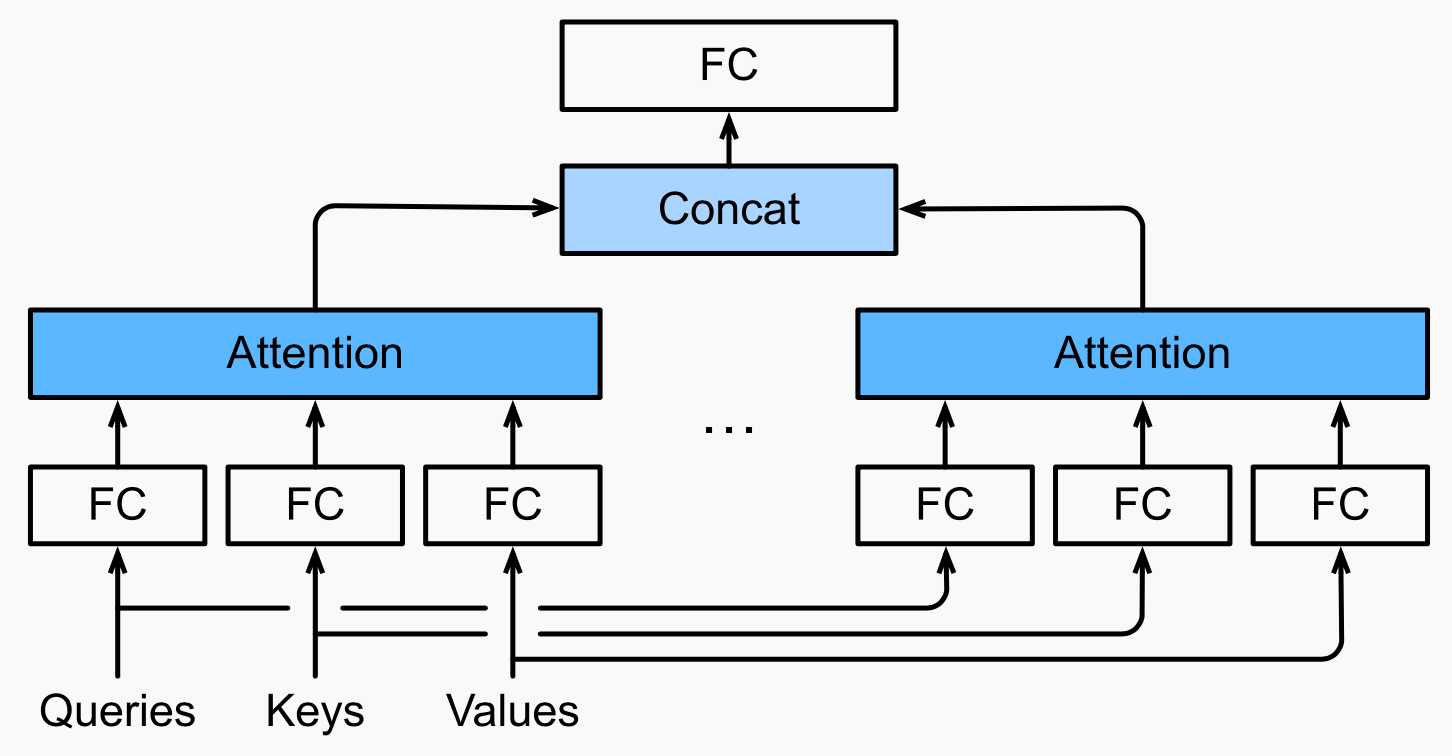
\includegraphics[height=4cm]{figures/multihead}
    \end{figure}
    \begin{itemize}
        \item Multiple attention modules: same architecture, different parameters
            \pause
        \item A \textbf{head}: one set of attention outputs
            \pause
        \item Concatenate all heads (increased output dimension)
        \item Linear projection to produce the final output
    \end{itemize}
\end{frame}

\begin{frame}
    {Matrix representation: input mapping}
    \begin{figure}
        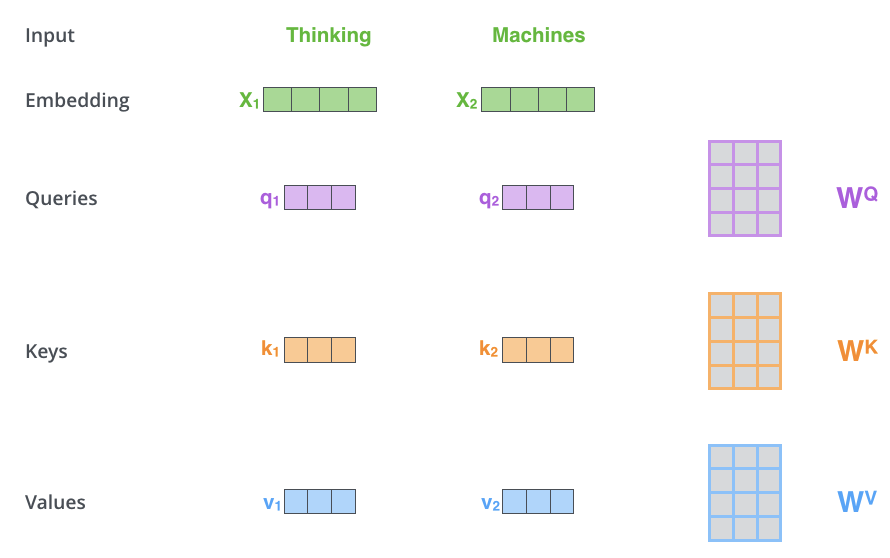
\includegraphics[height=7cm]{figures/self-attn-matrix.png}
        \caption{From \href{https://jalammar.github.io/illustrated-transformer}{The Illustrated Transformer}}
    \end{figure}
\end{frame}

\begin{frame}
    {Matrix representation: attention weights}
    Scaled dot product attention
    \begin{figure}
        \begin{subfigure}{.4\textwidth}
        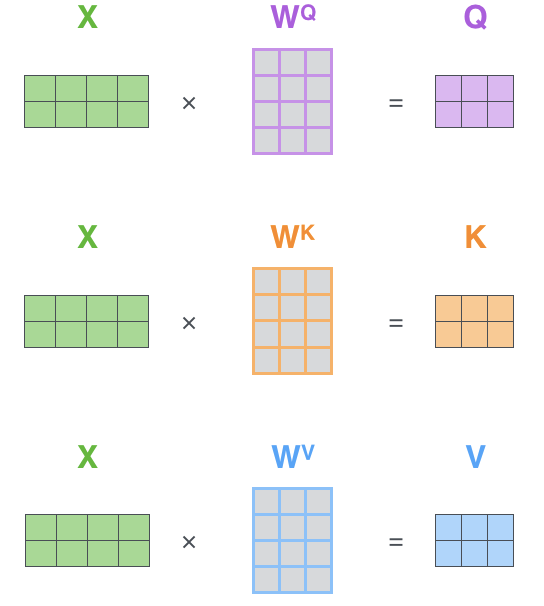
\includegraphics[height=4cm]{figures/scaled-attn}
        \end{subfigure}
        \begin{subfigure}{.5\textwidth}
        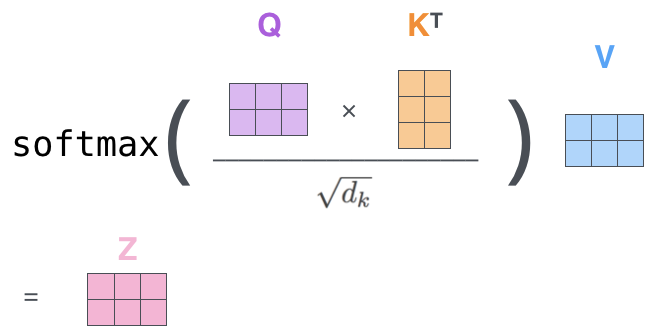
\includegraphics[height=3cm]{figures/scaled-attn-2}
        \end{subfigure}
        \caption{From \href{https://jalammar.github.io/illustrated-transformer}{The Illustrated Transformer}}
    \end{figure}
\end{frame}

\begin{frame}
    {Multi-head attention}
    \begin{figure}
        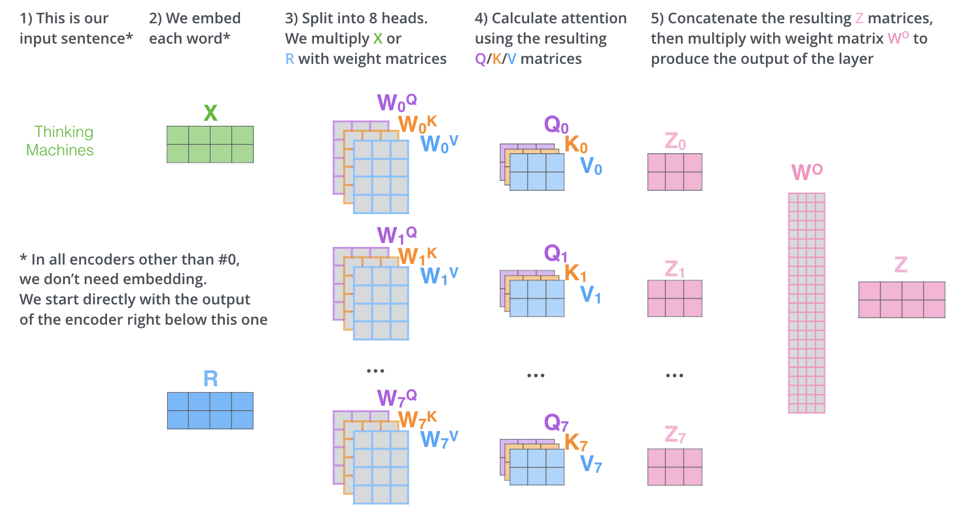
\includegraphics[width=.9\textwidth]{figures/multi-head-matrix}
        \caption{From \href{https://jalammar.github.io/illustrated-transformer}{The Illustrated Transformer}}
    \end{figure}
\end{frame}

\begin{frame}
    {Summary so far}
    \begin{wideitemize}
        \item Sequence modeling
            \begin{itemize}
                \item Input: a sequence of words
                \item Output: a sequence of contextualized embeddings for each word
                \item Models interaction among words
            \end{itemize}
            \pause
        \item Building blocks 
            \begin{itemize}
                \item Feed-forward / fully-connected neural network
                \item Recurrent neural network
                \item Self-attention
            \end{itemize}
            \pause
            \think{Which of these can handle sequences of arbitrary length?}
    \end{wideitemize}
\end{frame}

\section{Tranformer}

\begin{frame}
    {Overview}
    \begin{wideitemize}
        \item Use \blue{self-attention} as the core building block
        \item Vastly increased scalability (model and data size) compared to recurrence-based models
        \item Initially designed for machine translation (next week) 
            \begin{itemize}
                \item \textit{Attention is all you need}. Vaswani et al., 2017.
            \end{itemize}
        \item The backbone of today's large-scale models
        \item Extended to non-sequential data (e.g., images and molecules)
    \end{wideitemize}
\end{frame}

\begin{frame}
    {Transformer block}
    \begin{columns}
        \begin{column}{0.4\textwidth}
            \begin{figure}
                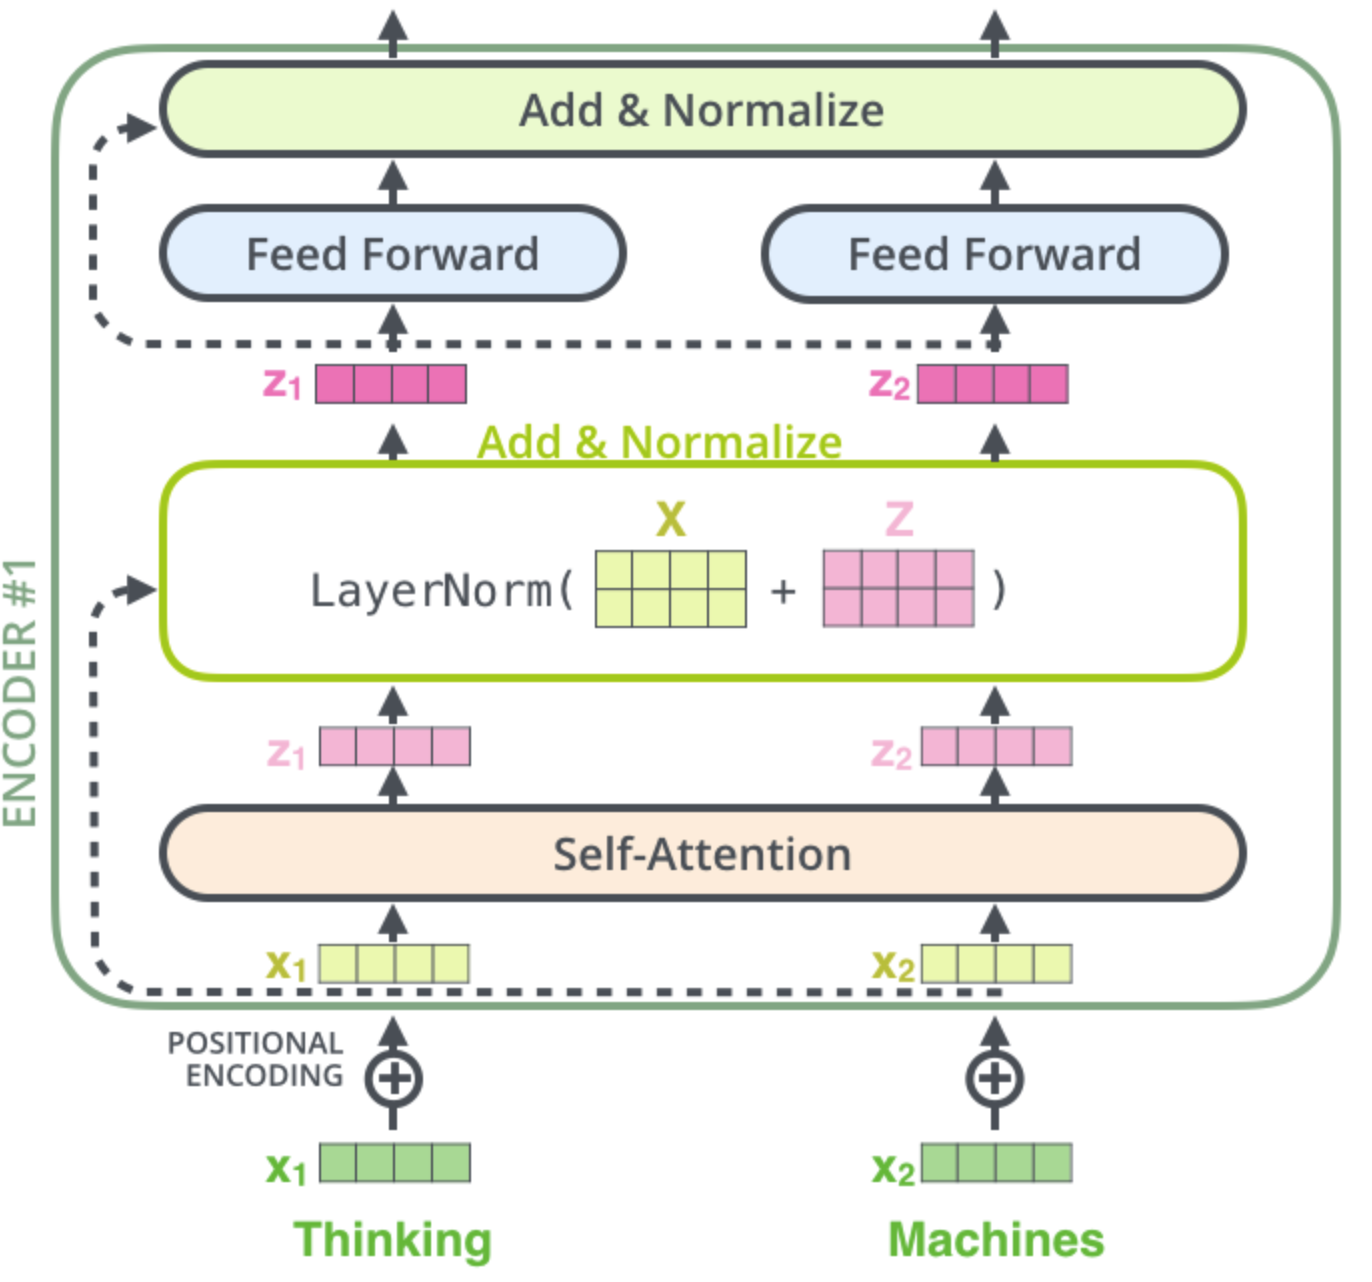
\includegraphics[width=\columnwidth]{figures/transformer-block}
                \caption{From \href{https://jalammar.github.io/illustrated-transformer}{The Illustrated Transformer}}
            \end{figure}
        \end{column}
        \begin{column}{0.6\textwidth}
            \begin{wideitemize}[<+->]
                \item Multi-head self-attention
                    \begin{itemize}
                        \item Capture dependence among input symbols
                    \end{itemize}
                \item Positional encoding 
                    \begin{itemize}
                        \item Capture the order of symbols 
                    \end{itemize}
                \item Residual connection and layer normalization 
                    \begin{itemize}
                        \item More efficient and stable optimization
                    \end{itemize}
            \end{wideitemize}
        \end{column}
    \end{columns}
\end{frame}

\begin{frame}
    {Position embedding}
    \textbf{Motivation}: model word order in the input sequence\\
    \textbf{Solution}: add a position embedding to each word
    \begin{figure}
        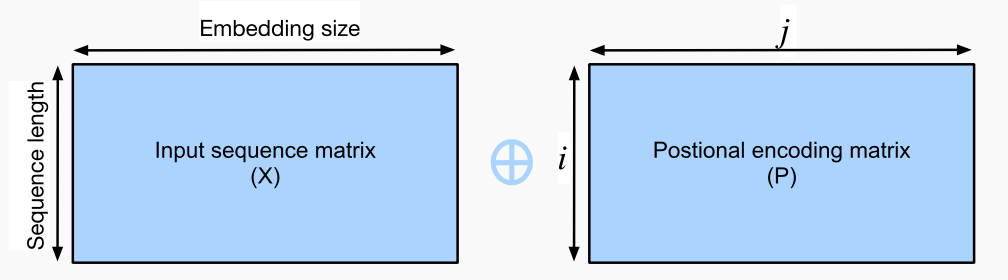
\includegraphics[height=3cm]{figures/position-embedding}
    \end{figure}

    Position embedding:\\
    \begin{itemize}
        \item Encode absolute and relative positions of a word
        \item Same dimension as word embeddings
        \item Learned or deterministic 
    \end{itemize}
\end{frame}

\begin{frame}
    {Sinusoidal position embedding}
    \textbf{Intuition}: continuous approximation of binary encoding of positions (integers)
    \vspace{-2em}

    \begin{figure}
        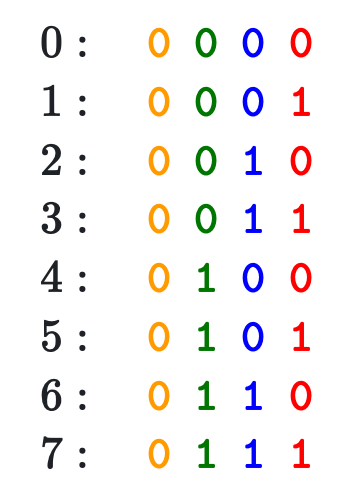
\includegraphics[height=4cm]{figures/binary}\pause
        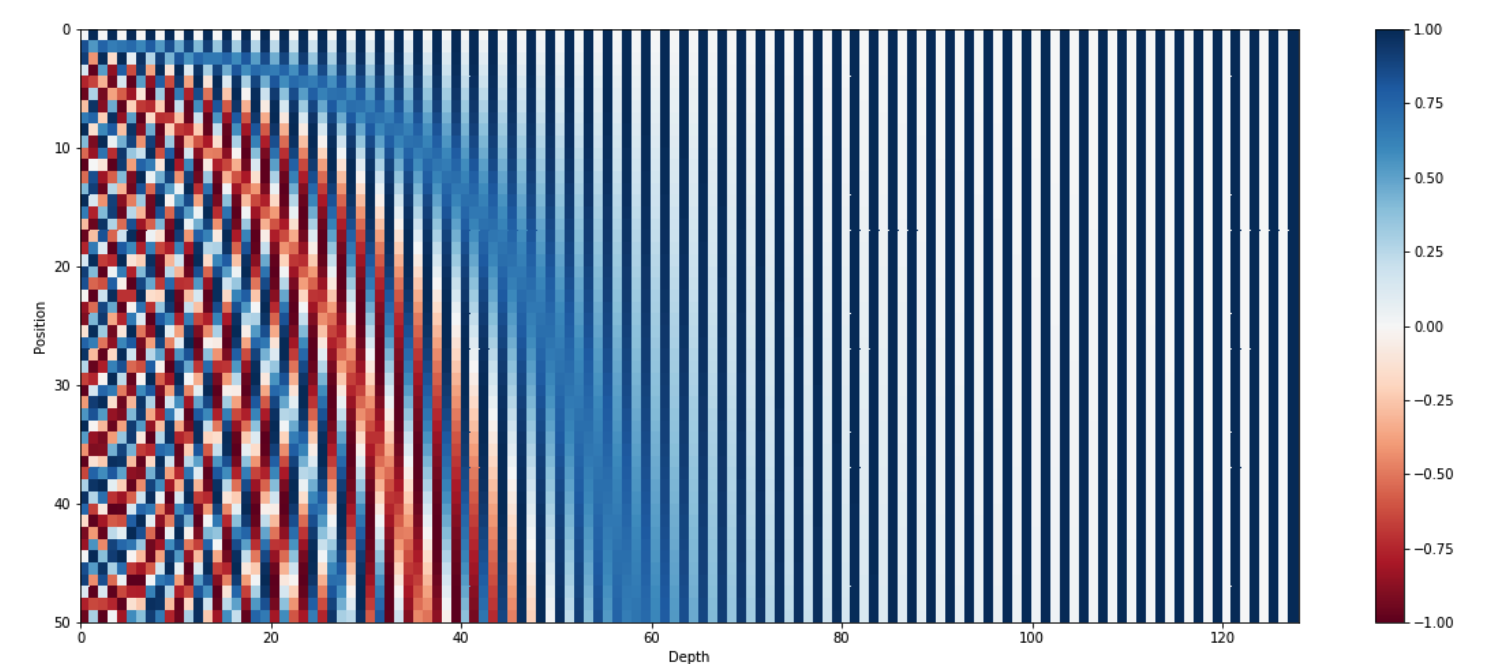
\includegraphics[height=4cm]{figures/sin}\pause
        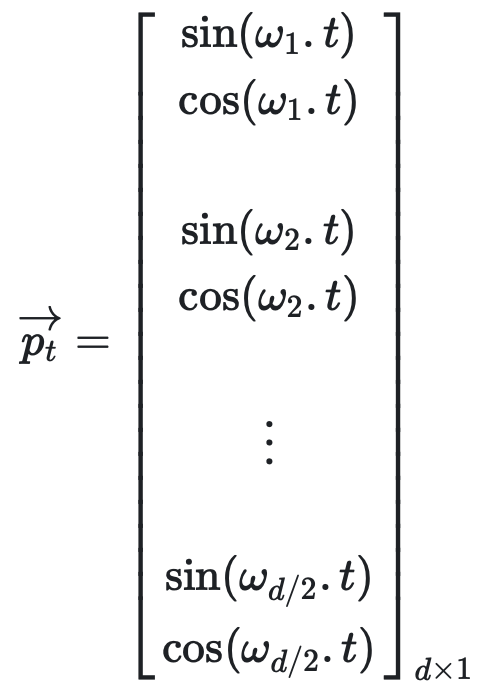
\includegraphics[height=4cm]{figures/pos}
        \caption{From \href{https://kazemnejad.com/blog/transformer_architecture_positional_encoding/}{Amirhossein Kazemnejad's Blog}}
    \end{figure}

    \vspace{-2em}
    \begin{align*}
        \omega_{k} = 1 / 10000^{\frac{2k}{d}}
    \end{align*}
\end{frame}

\begin{frame}
    {Learned position embeddings}

    Sinusoidal position embedding:\\
    \begin{itemize}
        \item Not learnable
        \item Can extrapolate to longer sequences but doesn't work well
    \end{itemize}
    \pause

    Learned absolute position embeddings (most common now):\\
    \begin{itemize}
        \item Consider each position as a word. Map positions to dense vectors: $W_{d\times n}\phi_{\text{one-hot}}(\text{pos})$
        \item Column $i$ of $W$ is the embedding of position $i$
            \pause
        \item Need to fix maximum position/length beforehand
        \item Cannot extrapolate to longer sequences
    \end{itemize}
\end{frame}

\begin{frame}
    {Residual connection}

    \textbf{Motivation}:\\
    \begin{wideitemize}
        \item Gradient explosion/vanishing is not RNN-specific!
        \item It happens to all very \blue{deep} networks (which are \red{hard to optimize}).
            \pause
        \item In principle, a deep network can always represent a shallow network (by setting higher layers to identity functions), thus it should be at least as good as the shallow network.
        \item For some reason, deep neural networks are bad at learning identity functions.
        \item How can we make it easier to recover the shallow solution?
    \end{wideitemize}
\end{frame}

\begin{frame}
    {Residual connection}

    \textbf{Solution}: \href{https://arxiv.org/pdf/1512.03385.pdf}{Deep Residual Learning for Image Recognition} [He et al., 2015]\\
    \begin{figure}
        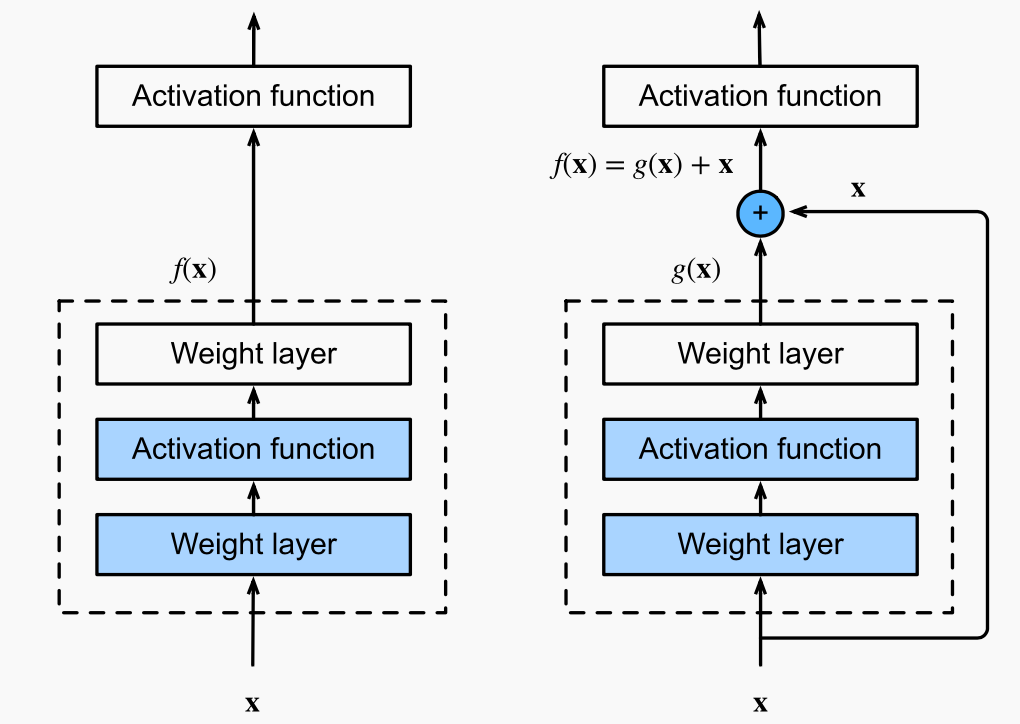
\includegraphics[height=5cm]{figures/residual}
    \end{figure}

    Without residual connection: learn $f(x) = x$.

    With residual connection: learn $g(x)=0$ (easier).
\end{frame}

\begin{frame}
    {Layer normalization}
    
    \begin{itemize}
        \item {\bf Problem}: inputs of a layer may shift during training
        \item {\bf Solution}: normalize (zero mean, unit variance) across features \mycite[https://arxiv.org/pdf/1607.06450.pdf]{[Ba et al., 2016]}
        \item Let $x=(x_1,\ldots,x_d)$ be the input vector (e.g., word embedding, previous layer output)
            \vspace{-1em}
            \begin{align*}
                \mathrm{LayerNorm}(x) &= \frac{x-\hat{\mu}}{\hat{\sigma}},\\
                \text{where} \; \hat{\mu} = \frac{1}{d}{\sum_{i=1}^d x_i}, &\quad \hat{\sigma}^2 = \frac{1}{d}{\sum_{i=1}^d (x_i-\hat{\mu})^2}
            \end{align*}
    \end{itemize}
    \pause
  
    \begin{columns}
        \begin{column}{0.5\textwidth}
            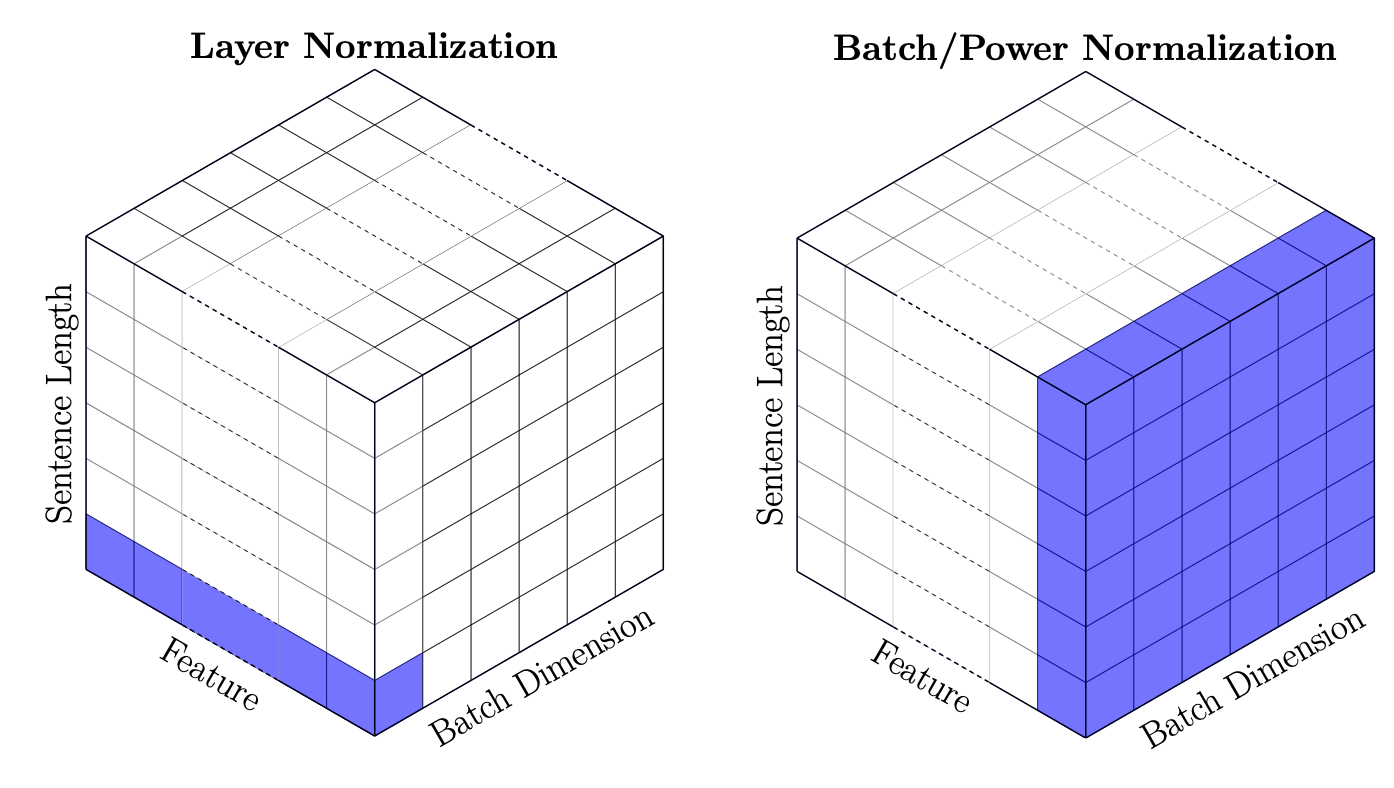
\includegraphics[height=4cm]{figures/batchnorm}
        \end{column}
        \begin{column}{0.5\textwidth}
    \begin{itemize}
    \item A deterministic transformation of the input
    \item Independent of train/inference and batch size
    \end{itemize}
        \end{column}
    \end{columns}
\end{frame}

\begin{frame}
    {Residual connection and layer normalization in Transformer}
    \begin{figure}
        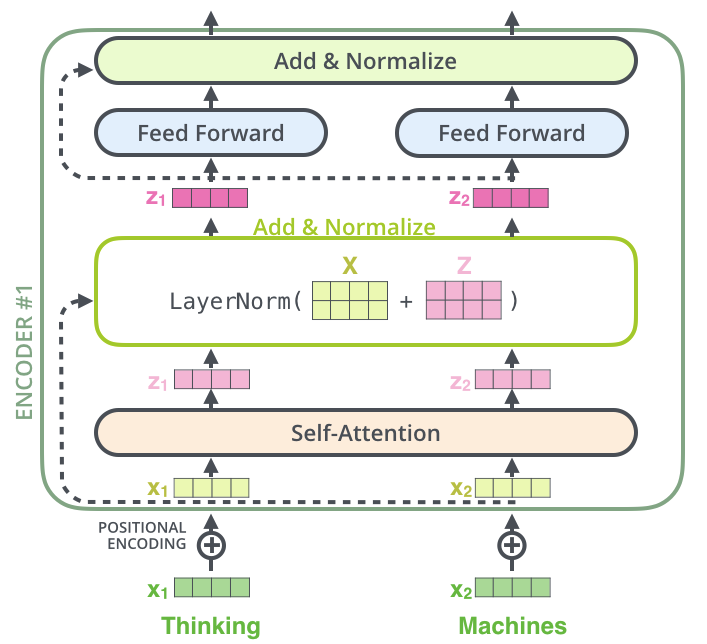
\includegraphics[height=5cm]{figures/add-norm}
    \end{figure}
    \vspace{-2em}
    \begin{itemize}
        \item Add (residual connection) \& Normalize (layer normalization) after each layer
        \item Position-wise feed-forward networks: same mapping for all positions
    \end{itemize}
\end{frame}

\begin{frame}
    {Summary}
    \begin{wideitemize}
        \item We have seen two families of models for sequences modeling: \textbf{RNNs} and \textbf{Transformers}
        \item Both take a sequence of (discrete) symbols as input and output a sequence of embeddings
        \item They are often called \textbf{encoders} and are used to represent text
        \item Transformers are dominating today because of its scalability
    \end{wideitemize}
\end{frame}

\end{document}
